%%%%%%%%%%%%%%%%%%%%%%%%%%%%%%%%%%%%%%%%%%%%%%%%%%%%%%%%%%%%%%%%%%%%%%%%%%%%%%%
\chapter{Medidas}
\label{Chap:Medidas}
%%%%%%%%%%%%%%%%%%%%%%%%%%%%%%%%%%%%%%%%%%%%%%%%%%%%%%%%%%%%%%%%%%%%%%%%%%%%%%%

\begin{fullwidth}
{\it Um dos principais objetivos da Física como ciência é determinar o resultado de experimentos não apenas qualitativamente, mas também quantitativamente. A realização de medidas está diretamente ligada a tal objetivo: para que possamos prever um resultado, precisamos de medidas de parâmetros relevantes do sistema e que servem de base para a previsão de novos valores através de um modelo matemático. Os valores previstos pelo modelo devem ser comparados com resultados experimentais, que ---~mais uma vez~--- devem ser medidos. Se as previsões concordarem com os resultados experimentais, o modelo deve ser submetido a mais testes; caso o modelo falhe, ele deve ser revisto. 

 O ato de realizar uma medição pode ser simples ou complexo, dependendo do tipo de medida a se realizar. Além disso, os valores obtidos estarão sempre sujeitos a erros que podem deturpar-los. Veremos abaixo alguns aspectos importantes para a determinação precisa de medidas.}
\end{fullwidth}

%%%%%%%%%%%%%%%%%%%%%%%%%%%%%%%%%%%
\section{Medição, tipos de medidas}
%%%%%%%%%%%%%%%%%%%%%%%%%%%%%%%%%%%

O processo de obtenção do valor de uma medida é denominado \emph{medição}. Tal processo consiste em comparar aquilo que se deseja medir com um padrão, obtendo o que se denomina como \emph{medida direta}, ou no cálculo de um valor a partir de um conjunto de medidas diretas, o que se denomina como \emph{medida indireta}.

Como exemplo de medida direta, podemos citar a determinação do comprimento de um objeto. Para obter o valor da medida, basta alinhar uma de suas extremidades ao zero de uma régua e verificarmos quantas marcas estão compreendidas no comprimento total do objeto. Temos, portanto, uma medida obtida através de uma comparação direta com um padrão de grandeza.

Algumas medidas, no entanto, não podem ser feitas de maneira direta ---~ou podem ser determinadas de maneira mais conveniente de forma indireta~---. Se necessitamos saber a área de uma folha retangular, basta verificarmos as medidas laterais e então multiplicá-las. Desta forma, estamos determinando a área de uma maneira \textbf{indireta}. Da mesma maneira, o volume de um paralelepípedo pode ser determinado de maneira indireta através do produto de suas três dimensões. Para um sólido irregular, no entanto, é mais conveniente mergulhá-lo em um líquido e verificar através de uma escala graduada impressa no recipiente que o comporta qual é o volume deslocado. Portanto, uma grandeza qualquer pode ser determinada de maneira direta ou indireta, sendo que a escolha de um ou outro tipo de método é uma questão de conveniência.

%%%%%%%%%%%%%%%%%%%%%%%%%%%%%%%%%%%%%%%%%%%%%%%%%%%%%%%%%%%%
\section{Tipos de equipamentos, algarismos significativos}
%%%%%%%%%%%%%%%%%%%%%%%%%%%%%%%%%%%%%%%%%%%%%%%%%%%%%%%%%%%%

Os equipamentos de medida podem ser divididos em dois tipos:
\begin{description}
	\item[Analógicos] Os equipamentos analógicos são aqueles que permitem que realizemos uma estimativa de valores entre duas marcas quaisquer de sua escala. São exemplos deste tipo de equipamento réguas, velocímetros de ponteiro, relógios de ponteiros, etc.

	\item[Não-analógicos] Equipamentos que não permitem a estimativa de valores são classificados como não-analógicos: nessa categoria se incluem os equipamentos digitais e aqueles dotados de escalas auxiliares. Nos equipamentos digitais, os dados da medida são mostrados através de um visor digital que permite a leitura direta dos valores numéricos\footnote[][-6cm]{Em equipamentos digitais que verificam o valor de uma quantidade que costuma sofrer pequenas variações em torno de um valor, os aparelhos geralmente realizam uma série de medidas durante um certo intervalo de tempo e mostram somente o valor médio de tais medidas. Um exemplo disso são os velocímetros digitais: devido a pequenas variações de velocidade que ocorrem durante a condução, o processo descrito acima deve ser realizado visando mostrar um número que sofra variações menos frequentes, distraindo menos o condutor.}. Já os equipamentos dotados de escala auxiliar ---~também conhecida como nônio ou vernier~--- possibilitam a leitura em uma escala analógica principal, porém com a leitura da subdivisão da escala principal na escala auxiliar. Como a escala auxiliar tem divisões muito ``finas'', no entanto, não é possível estimar digitos menores do que a menor divisão da escala auxiliar.
\end{description}
%
Vamos tratar as medidas realizadas por cada tipo de equipamento separadamente nas seções seguintes. Trataremos também a questão de \emph{algarismos significativos} de uma medida.
\begin{marginfigure}[-3cm]
	\includegraphics[width=\textwidth]{Ilustrations/Regua.png}
	\caption{Exemplo de equipamento analógico: réguas.}
\end{marginfigure}
%
\begin{figure}
	\centering
	\includegraphics[width=0.7\textwidth]{Ilustrations/Balanca.png}
	\caption{Equipamentos eletrônicos geralmente utilizam um visor digital para expressar os valores medidos. Na figura, uma balança digital.}
\end{figure}
%
\begin{marginfigure}[-1cm]
	\includegraphics[width=\textwidth]{Ilustrations/Dilatometro.png}
	\caption{Equipamentos com ponteiros são exemplos comuns de equipamentos analógicos. Na figura temos um dilatômetro, equipamento utilizado para verificar pequenas variações de tamanho características de dilatação térmica (uma volta completa representa uma variação de \np[mm]{1,0}).}
\end{marginfigure}
%

%%%%%%%%%%%%%%%%%%%%%%%%%%%%%%%%%%%%%%%%%%%%%%%%%%%%%%
\subsection{Medidas realizadas com equipamentos analógicos}
\label{Sec:MedEquipAnalog}
%%%%%%%%%%%%%%%%%%%%%%%%%%%%%%%%%%%%%%%%%%%%%%%%%%%%%%

Suponhamos que precisamos usar uma régua milimetrada para realizar uma medida de uma haste. O equipamento em questão foi elaborado de tal forma que um metro está subdividido em 1000 partes, isto é, a menor distância entre as marcações é de 1 mm.

\begin{figure*}[!hb]
\centering
\begin{tikzpicture}

% Régua
	\foreach \x in {0.0, 0.1, ..., 13.7}
		\draw (\x,0) -- (\x,0.5);

	\foreach \x in {0, 0.5, ..., 13.5}
		\draw (\x,0) -- (\x,0.7);

	\draw (0,0) -- (0,1) node[anchor=south] {0};
	\foreach \x in {1, 2, ..., 13}
		\draw (\x,0) -- (\x,1) node[anchor=south] {\x};
		
	\draw[pattern=north west lines](0,-0.1) rectangle (10.83,-1.1);

\end{tikzpicture}
\caption{Medindo uma haste com uma régua milimetrada.\label{Fig:MedindoHasteComUmaRegua}}
\end{figure*}

Para realizar a medição, alinhamos uma extremidade da régua ---~aquela que contém o zero~--- com uma extremidade da haste e verificamos a outra extremidade desse corpo (veja a Figura~\ref{Fig:MedindoHasteComUmaRegua}). Vemos que a segunda extremidade passa da marca dos \np[m]{10,8} centímetros, mas não chega à marca de \np[cm]{10,9}. O valor da medida do comprimento $\ell$ da haste está em algum ponto entre os valores correspondentes às duas marcas:
\begin{equation}
     \np[cm]{10,8} < \ell < \np[cm]{10,9}.
\end{equation}

\noindent{}Note, no entanto, que \emph{podemos estimar mais um algarismo}. Se, por exemplo, a extremidade da haste está próxima da metade da distância entre as duas marcas da régua, porém antes dela, poderíamos estimar um valor 3 (isto é, três décimos da distância entre as duas subdivisões). Assim, podemos expressar a medida como,
\begin{equation}
     \ell = \np[cm]{10,83}.
\end{equation}

Poderíamos realizar uma estimativa com mais casas após o 3, mas a validade dela seria duvidosa: se já não temos certeza sobre a medida ser 3 (poderia ser 2 ou 4, em escalas menores é difícil efetuar uma estimativa), não temos ganho de informação algum em denotar mais algarismos após o 3. Ao conjunto de algarismos que temos certeza (pois foram verificados no instrumento) e ao algarismo estimado, damos o nome de \emph{algarismos significativos}. O último algarismo também é conhecido como \emph{algarismo duvidoso}, pois seu valor pode mudar ao se utilizar um equipamento de medida mais preciso.

Em casos onde realizamos uma medida que coincide exatamente com uma marca, devemos considerar que o equipamento permitiria expressar divisões menores, se fosse o caso. Se, por exemplo, ao medirmos a haste com a régua/trena mencionada, a extremidade coincidir com a marca de \np[cm]{10,8}, devemos expressar a medida como
\begin{equation}
	\ell = \np[cm]{10,80},
\end{equation}
%
pois sabemos determinamos que o algarismo estimado é zero (pois se aparentemente coincide com a marca, não a ultrapassa em quantidade apreciável).

A estimativa do último dígito é uma característica importante das escalas analógicas e deve sempre ser realizada e o dígito correspondente deve ser registrado na medida. Note ainda que o número de algarismos significativos das medidas registradas por um dado equipamento \emph{não é constante}. Por exemplo, as medidas
\begin{align}
	\ell_1 &= \np[cm]{0,75} \\
	\ell_2 &= \np[cm]{1,38} \\
	\ell_3 &= \np[cm]{11,50},
\end{align}
%
são todas medidas que podem ser obtidas usando uma régua/trena milimetrada, porém têm 2, 3, e 4 algarismos significativos, respectivamente. Por outro lado, verificamos que \emph{o número de casas decimais é sempre o mesmo}: todas as medidas possuem duas casas decimais quando expressamos as medidas em centímetros.

%%%%%%%%%%%%%%%%%%%%%%%%%%%%%%%%%%%%%%%%%%%%%%
\paragraph{Leitura de um micrômetro analógico}
%%%%%%%%%%%%%%%%%%%%%%%%%%%%%%%%%%%%%%%%%%%%%%

\begin{figure}[t] \forceversofloat
	\centering
	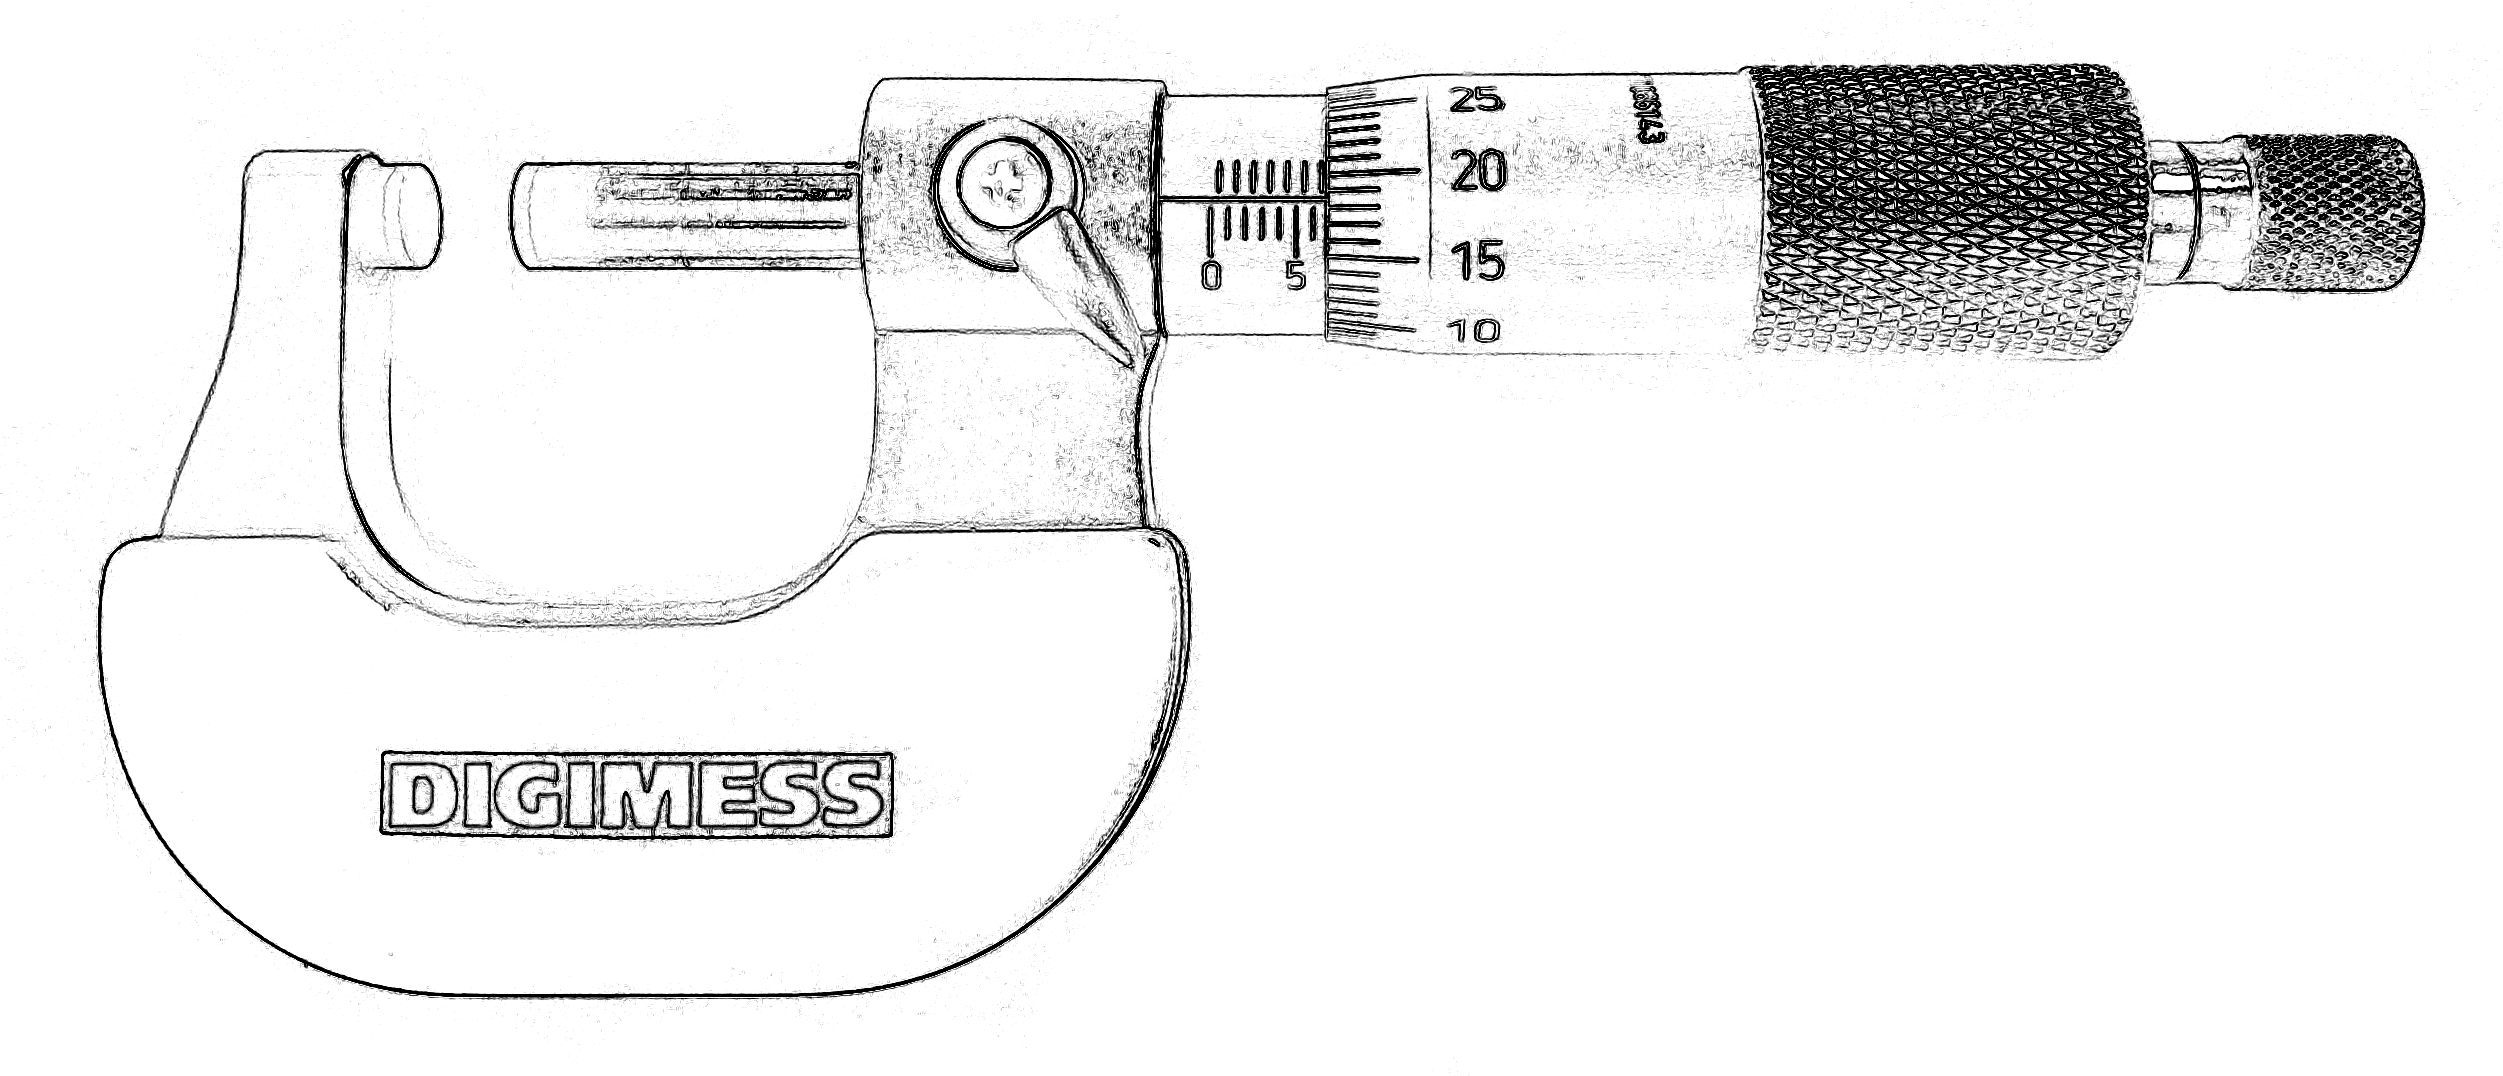
\includegraphics[width=\textwidth]{Ilustrations/Micrometro_sem_obj.png}
	\caption{Um micrômetro pode ter ou não uma escala auxiliar: na figura, temos um exemplo em que não há escala auxiliar e por isso permite que um dígito seja estimado nas leituras.\label{Fig:MicrometroSemObj}}
\end{figure}

A escala de um micrômetro pode sofrer alguma variação entre diferentes modelos. Na Figura~\ref{Fig:MicrometroSemObj} temos um micrômetro em que a cada duas voltas do ``tambor'' (a parte cilíndrica externa) temos um afastamento de 1 mm da haste em relação ao apoio oposto. Além disso, verificamos que a linha central aponta um número no tambor.

Para melhor entendermos como realizar a medida, podemos observar a Figura~\ref{Fig:DetalheEscalaMicrometro}. Podemos dividir a medida em duas partes: a leitura da escala horizontal na figura, e a leitura da escala vertical (a do tambor).

\begin{figure}
\centering
\begin{tikzpicture}[scale=1.7]

	\pgfmathsetmacro{\reading}{23.282} % leitura em mm
	
	\pgfmathsetmacro{\decimalpart}{\reading - int(\reading)}  % Extract decimal part
	\pgfmathsetmacro{\scaleddecimal}{\decimalpart * 100}  % Multiply by 100
	\pgfmathsetmacro{\yshift}{mod(\scaleddecimal, 50)}
	\pgfmathsetmacro{\clipsize}{\reading + 10}

	\clip (-0.5,1) rectangle (\clipsize mm,-1);
	
% Escala principal

	\draw (-0.4,0) -- (7,0);
	
	\foreach \x in {0.0, 0.1, ..., 7.0}
		\draw (\x,-0.05) -- (\x,-0.15);

	\foreach \x in {0, 5, ..., 70}
		\draw (\x mm,-0.05) -- (\x mm,-0.3)node[below]{\tiny \x};

	\foreach \x in {0.05, 0.15, ..., 7.0}
		\draw (\x,0.05) -- (\x,0.15);

% Escala auxiliar
	\begin{scope}[xshift=\reading mm]
		\fill[white] (0,-1) rectangle (1,1);
		\draw[gray] (0,-1) -- (0,1);
		
		\begin{scope}[yshift=-\yshift mm]
			\foreach \y in {0, 1, ...,49}
				\draw (0,\y mm) -- (2 mm,\y mm);

			\foreach \y in {0, 5, ..., 49}{
				%\pgfmathsetmacro{\newy}{int(\y + 10)}
				\draw (0,\y mm) -- (4 mm,\y mm) node[right]{\tiny \y};
			}
			
			\foreach \y in {0, 1, ..., 50}{
				\pgfmathsetmacro{\newy}{int(\y + 50)}
				\draw (0,\newy mm) -- (2 mm,\newy mm);
			}

			\foreach \y in {0, 5, ..., 50}{
				\pgfmathsetmacro{\newy}{int(\y + 50)}
				\draw (0,\newy mm) -- (4 mm,\newy mm) node[right]{\tiny \y};
			}
			
			\foreach \y in {0, 1, ..., 49}{
				\pgfmathsetmacro{\newy}{int(\y - 50)}
				\draw (0,\newy mm) -- (2 mm,\newy mm);
			}
			\foreach \y in {0, 5, ..., 49}{
				\pgfmathsetmacro{\newy}{int(\y - 50)}
				\draw (0,\newy mm) -- (4 mm,\newy mm) node[right]{\tiny \y};
			}
		\end{scope}
	
		\fill[color=white,path fading=south] (0,0) rectangle (1,1.2);
		\fill[color=white,path fading=north] (0,0) rectangle (1,-1.2);
		
	\end{scope}
\end{tikzpicture}
\caption{Escala de um micrômetro analógico.\label{Fig:DetalheEscalaMicrometro}}
\end{figure}

A leitura da escala horizontal é feita através da borda do tambor. Nas marcações abaixo da linha central, temos os milímetros inteiros; já nas marcações acima da linha temos os ``meios-milímetros''.\footnote{Como um milímetro é equivalente a duas voltas, precisamos contar de meio em meio milímetro.} Notamos na parte inferior que a marca mais à direita visível é a de \np[mm]{23}. Portanto, temos para a medida
\begin{equation}
	\ell = 23{,}\dots
\end{equation}
%
Para determinarmos a leitura dos valores após a vírgula, usamos a linha central como indicador para lermos a escala do tambor. No caso da \ref{Fig:DetalheEscalaMicrometro}, vemos que a linha indica um valor que excede a marca de número 28; notamos ainda que podemos fazer uma estimativa de aproximadamente 2 décimos da distância entre duas marcas. Logo, a leitura do tambor equivale a \np[mm]{0,282}. Finalmente, podemos escrever a medida final como
\begin{equation}
	\ell = 23{,}282\,\text{mm}.
\end{equation}

Um caso marginalmente mais complexo é o mostrado na Figura~\ref{Fig:DetalheEscalaMicrometro2}. Nela observamos que a marca mais à direita visível corresponde à de \np[mm]{37,5} (note a marca que aparece acima da linha central). A leitura da escala do tambor nos dá \np[mm]{0,292}. Assim,\footnote[][-1.5cm]{Essa equação não representa uma soma de medidas, mas sim a composição das parcelas de uma mesma medida, por isso não precisamos levar em conta regras de algarismos significativos para a soma. Outra maneira de pensar é que temos certeza absoluta acerca do valor da primeira parcela, então sua precisão é infinita, tornando a segunda parcela a responsável por definir o número de casas após a vírgula para o resultado.} 
\begin{align}
	\ell &= \np[mm]{37,5} + \np[mm]{0,292} \\
	&= \np[mm]{37,792}.
\end{align}

\begin{figure}
\centering
\begin{tikzpicture}[scale=1.7]

	\pgfmathsetmacro{\reading}{37.792} % leitura em mm
	
	\pgfmathsetmacro{\decimalpart}{\reading - int(\reading)}  % Extract decimal part
	\pgfmathsetmacro{\scaleddecimal}{\decimalpart * 100}  % Multiply by 100
	\pgfmathsetmacro{\yshift}{mod(\scaleddecimal, 50)}
	\pgfmathsetmacro{\clipsize}{\reading + 10}

	\clip (-0.5,1) rectangle (\clipsize mm,-1);
	
% Escala principal

	\draw (-0.4,0) -- (7,0);
	
	\foreach \x in {0.0, 0.1, ..., 7.0}
		\draw (\x,-0.05) -- (\x,-0.15);

	\foreach \x in {0, 5, ..., 70}
		\draw (\x mm,-0.05) -- (\x mm,-0.3)node[below]{\tiny \x};

	\foreach \x in {0.05, 0.15, ..., 7.0}
		\draw (\x,0.05) -- (\x,0.15);

% Escala auxiliar
	\begin{scope}[xshift=\reading mm]
		\fill[white] (0,-1) rectangle (1,1);
		\draw[gray] (0,-1) -- (0,1);
		
		\begin{scope}[yshift=-\yshift mm]
			\foreach \y in {0, 1, ...,49}
				\draw (0,\y mm) -- (2 mm,\y mm);

			\foreach \y in {0, 5, ..., 49}{
				%\pgfmathsetmacro{\newy}{int(\y + 10)}
				\draw (0,\y mm) -- (4 mm,\y mm) node[right]{\tiny \y};
			}
			
			\foreach \y in {0, 1, ..., 50}{
				\pgfmathsetmacro{\newy}{int(\y + 50)}
				\draw (0,\newy mm) -- (2 mm,\newy mm);
			}

			\foreach \y in {0, 5, ..., 50}{
				\pgfmathsetmacro{\newy}{int(\y + 50)}
				\draw (0,\newy mm) -- (4 mm,\newy mm) node[right]{\tiny \y};
			}
			
			\foreach \y in {0, 1, ..., 49}{
				\pgfmathsetmacro{\newy}{int(\y - 50)}
				\draw (0,\newy mm) -- (2 mm,\newy mm);
			}
			\foreach \y in {0, 5, ..., 49}{
				\pgfmathsetmacro{\newy}{int(\y - 50)}
				\draw (0,\newy mm) -- (4 mm,\newy mm) node[right]{\tiny \y};
			}
		\end{scope}
	
		\fill[color=white,path fading=south] (0,0) rectangle (1,1.2);
		\fill[color=white,path fading=north] (0,0) rectangle (1,-1.2);
		
	\end{scope}
\end{tikzpicture}
\caption{Escala de um micrômetro analógico.\label{Fig:DetalheEscalaMicrometro2}}
\end{figure}

%%%%%%%%%%%%%%%%%%%%%%%%%%%%%%%%%%%%%%%%%%%%%%%%%%%%%%%%%%%%%%%
\subsection{Medidas realizadas com equipamentos não-analógicos}
%%%%%%%%%%%%%%%%%%%%%%%%%%%%%%%%%%%%%%%%%%%%%%%%%%%%%%%%%%%%%%%

%\pagebreak

\begin{figure*}[b]
	\includegraphics[width=\textwidth]{Ilustrations/Paquimetro.png}
	\caption{O paquímetro é um exemplo de equipamento \emph{não-analógico}, pois é dotado de escala auxiliar (nônio).}
\end{figure*}

No caso de equipamentos não-analógicos, podemos subdividi-los em equipamentos digitais e em equipamentos dotados de escalas auxiliares. No caso do primeiro, a medida consiste em ler os números mostrados através de um visor. Todos os algarismos mostrados são significativos ---~exceto aqueles que simplesmente posicionam a vírgula, veja a seção seguinte~---. Nesse caso, o último é o algarismo duvidoso, pois, novamente, seu valor poderia ser diferente se utilizássemos um equipamento mais preciso para realizar a medida.

No caso de equipamentos dotados de escalas auxiliares, apesar de não realizarmos a leitura de um visor digital, também não realizamos estimativas. Nesse caso realizamos a leitura a partir da escala auxiliar e, devido à precisão de tal escala, não conseguimos realizar estimativas. Novamente, todos os algarismos lidos são significativos\footnote{Exceto os que posicionam a vírgula, veja a Seção~\ref{Sec:UnidadesAlgSigNotacaoCientifica} para mais informações.}, sendo que o último é denominado duvidoso devido ao fato de que pode mudar ao se utilizar um equipamento mais preciso.

\pagebreak
%%%%%%%%%%%%%%%%%%%%%%%%%%%%%%%%%%%%%%%%%%%%
\paragraph{Funcionamento da escala auxiliar}
%%%%%%%%%%%%%%%%%%%%%%%%%%%%%%%%%%%%%%%%%%%%

\begin{marginfigure}[2 cm]
\centering
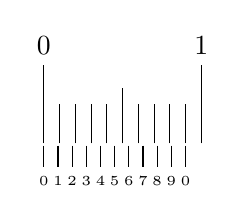
\begin{tikzpicture}
	
% escala principal
	\draw (0,0) -- (0,1) node[anchor=south] {0};
	\foreach \x in {0.2, 0.4, 0.6, 0.8, 1.2, 1.4, 1.6, 1.8}
		\draw (\x,0) -- (\x,0.5);
	\draw (1.0,0) -- (1.0,0.7);
	\draw (2,0) -- (2,1) node[anchor=south] {1};

% escala auxiliar
	\foreach \x [count=\xi from=0] in {0, 0.18, ..., 1.62}
		\draw (\x,-0.03) -- (\x,-0.3) node[anchor=north] {\tiny \xi};
	\draw (1.8,-0.03) -- (1.8, -0.3) node[anchor=north] {\tiny 0};
\end{tikzpicture}
\caption{Escala de um equipamento dotado de escala auxiliar. A escala superior é a principal, enquanto a inferior é a auxiliar.\label{Fig:NonioFechado}}
\end{marginfigure}


Em um equipamento dotado de uma escala auxiliar ---~como um paquímetro, por exemplo~---, as medidas devem ser feitas utilizando-se a posição na escala principal do zero da escala auxiliar. Na Figura~\ref{Fig:NonioFechado} vemos uma representação das escalas de leitura típicas de um equipamento dotado de escala auxiliar: a escala maior é a principal, enquanto a menor, móvel, é a auxiliar.

A ideia por trás da escala auxiliar é bastante simples: 
\begin{itemize}
	\item Tomamos a menor divisão da escala principal e a subdividimos em $n$ partes;
	\item Fazemos uma escala auxiliar onde a menor divisão é a largura de $n-1$ partes;
\end{itemize}
%
Assim, temos que\footnote{Considerando que as escalas principal e auxiliar estão ligadas à pinça do paquímetro, o deslocamento da escala auxiliar equivale à medida da distância entre as faces de medição.}
\begin{itemize}
	\item se a escala auxiliar estiver deslocada para a direita pela largura de uma parte, a marca imediatamente à direita do zero da escala auxiliar estará alinhado com a marca imediatamente à direita da do zero da escala principal;
	\item se a marca do zero estiver deslocada por duas vezes a largura de uma parte, a segunda marca à direita do zero da escala auxiliar se alinhará à segunda marca à direita do zero da escala principal;
\end{itemize}
%
e assim por diante. Dessa forma, podemos realizar uma leitura em que a resolução é uma subdivisão da menor divisão da escala principal, bastando verificar o alinhamento entre as marcas das escalas.

\begin{marginfigure}
\centering
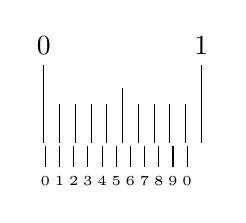
\begin{tikzpicture}

% escala principal
	\draw (0,0) -- (0,1) node[anchor=south] {0};
	\foreach \x in {0.2, 0.4, 0.6, 0.8, 1.2, 1.4, 1.6, 1.8}
		\draw (\x,0) -- (\x,0.5);
	\draw (1.0,0) -- (1.0,0.7);
	\draw (2,0) -- (2,1) node[anchor=south] {1};

% escala auxiliar
	\foreach \x [count=\xi from=0] in {0.02, 0.20, ..., 1.64}
		\draw (\x,-0.03) -- (\x,-0.3) node[anchor=north] {\tiny \xi};
	\draw (1.82,-0.03) -- (1.82, -0.3) node[anchor=north] {\tiny 0};
\end{tikzpicture}
\caption{Escala auxiliar deslocada para a direita por um décimo da largura da menor divisão da escala principal. Note que a marca número 1 da escala auxiliar está alinhada com a primeira marca à direita do zero da escala principal. \label{Fig:NonioAbertoUmaParte}}
\end{marginfigure}

\begin{marginfigure}
\centering
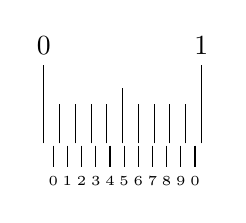
\begin{tikzpicture}

% escala principal
	\draw (0,0) -- (0,1) node[anchor=south] {0};
	\foreach \x in {0.2, 0.4, 0.6, 0.8, 1.2, 1.4, 1.6, 1.8}
		\draw (\x,0) -- (\x,0.5);
	\draw (1.0,0) -- (1.0,0.7);
	\draw (2,0) -- (2,1) node[anchor=south] {1};

% escala auxiliar
	\foreach \x [count=\xi from=0] in {0.12, 0.30, ..., 1.75}
		\draw (\x,-0.03) -- (\x, -0.3) node[anchor=north] {\tiny \xi};
	\draw (1.92,-0.03) -- (1.92, -0.3) node[anchor=north] {\tiny 0};
\end{tikzpicture}
\caption{Escala auxiliar deslocada por 6 décimos da largura da menor divisão da escala superior. Note o alinhamento da marca número 6.\label{Fig:NonioAbertoSeisPartes}}
\end{marginfigure}

Nas Figuras \ref{Fig:NonioAbertoUmaParte} e \ref{Fig:NonioAbertoSeisPartes} temos dois exemplos concretos de medidas utilizando a escala auxiliar da Figura~\ref{Fig:NonioFechado}. A escala auxiliar de tais figuras foi construída de forma que a menor divisão da escala principal foi subdividida em 10 partes. Tomando 9 partes, construímos a menor divisão da escala auxiliar. Assim, 
\begin{itemize}
	\item se a escala auxiliar for deslocada para a direita por uma distância equivalente a um décimo da largura da menor divisão da escala principal, temos que a marca à direita do zero da escala auxiliar se alinhará à marca à direita do zero da escala principal, que é situação da Figura~\ref{Fig:NonioAbertoUmaParte};
	\item na Figura~\ref{Fig:NonioAbertoSeisPartes} o zero da escala auxiliar está deslocado em seis partes para a direita, o que leva ao alinhamento da marca número 6 da escala auxiliar com a sexta marca à direita do zero da escala principal.
\end{itemize}

%%%%%%%%%%%%%%%%%%%%%%%%%%%%%%%%%%%%%%%%%%%%%%%%%%%%%%%%
\paragraph{Tomando medidas utilizando a escala auxiliar}
%%%%%%%%%%%%%%%%%%%%%%%%%%%%%%%%%%%%%%%%%%%%%%%%%%%%%%%%

A Figura~\ref{Fig:NonioMedida} retrata uma medida tomada com um paquímetro cuja menor divisão da escala principal é de um milímetro e no qual a menor divisão da escala auxiliar é de 9/10 da largura da menor divisão da escala principal. Para tomar a medida, fazemos o seguinte:
%
\begin{marginfigure}
\centering
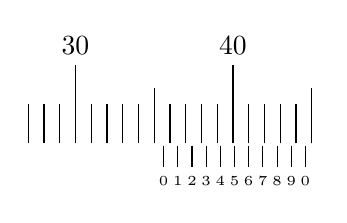
\begin{tikzpicture}

% escala principal
	\foreach \x in {-0.6, -0.4, ..., 3.2}
		\draw (\x,0) -- (\x,0.5);
	\draw (0,0) -- (0,1) node[anchor=south] {30};
	\draw (1.0,0) -- (1.0,0.7);
	\draw (2,0) -- (2,1) node[anchor=south] {40};
	\draw (3.0,0) -- (3.0,0.7);

% escala auxiliar
	\foreach \x [count=\xi from=0]in {1.12, 1.30, ..., 2.75} % última marca em 2.74
		\draw (\x, -0.03) -- (\x,-0.3) node[anchor=north] {\tiny \xi};
		
	\draw (2.92,-0.03) -- (2.92,-0.3) node[anchor=north] {\tiny 0};
	
\end{tikzpicture}
\caption{Exemplo de medida em um equipamento dotado de escala auxiliar.\label{Fig:NonioMedida}}
\end{marginfigure}
%
\begin{enumerate}
	\item Efetuamos a leitura na escala principal através do zero da escala auxiliar. Consideramos a marcação imediatamente à esquerda do zero da escala auxiliar. Nesse caso temos \np[mm]{35}.
	\item Verificamos qual é a marca da escala auxiliar que tem o melhor alinhamento com uma marca da escala principal. Nesse caso, temos que tal marca é a de número 6.
	\item Como dividimos a menor divisão da escala principal em 10 partes para elaborar a escala auxiliar, ao alinharmos a sexta marca da escala auxiliar, temos 6/10 de um milímetro, ou seja, \np[mm]{0,6}.
	\item Somando essas duas contribuições, temos que a medida é \np[mm]{35,6}.
\end{enumerate}
%
Veja que, na prática, \emph{basta ler a escala principal através do zero da escala auxiliar, inserir uma vírgula, e anotar o número da marca na escala auxiliar que está alinhada à marca da escala principal}. Note ainda que o zero da direita na escala auxiliar serve para ajudar a verificar o alinhamento do zero da esquerda, pois ambos ficam alinhados ao mesmo tempo.

\begin{figure*}\forcerectofloat
\centering
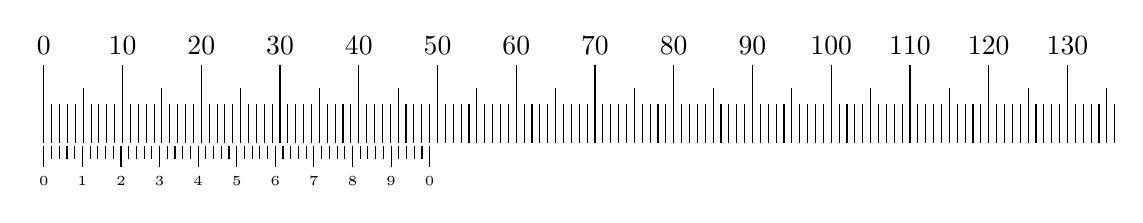
\begin{tikzpicture}

% Escala principal
	\foreach \x in {0.0, 0.1, ..., 13.7}
		\draw (\x,0) -- (\x,0.5);

	\foreach \x in {0, 0.5, ..., 13.5}
		\draw (\x,0) -- (\x,0.7);

	\draw (0,0) -- (0,1) node[anchor=south] {0};
	\foreach \x in {1, 2, ..., 13}
		\draw (\x,0) -- (\x,1) node[anchor=south] {\x0};

% Escala auxiliar
	\foreach \x in {0.000, 0.098, ..., 4.9}
		\draw (\x,-0.03) -- (\x,-0.2);

	\foreach \x [count=\xi from 0] in {0, 0.490, ..., 4.9}
		\draw (\x,-0.03) -- (\x,-0.3) node[anchor=north] {\tiny \xi};
	
	\draw (4.900,-0.03) -- (4.900,-0.3) node[anchor=north] {\tiny 0};

\end{tikzpicture}
\caption{Escalas de um paquímetro milimetrado em que a menor divisão da escala principal é subdividida em 50 partes para elaborar a escala auxiliar.}
\label{Fig:Paquimetro}
\end{figure*}

%%%%%%%%%%%%%%%%%%%%%%%%%%%%%%%%%%%%%%%%%%%%%%%%%%%%%%%%%%%%%
\paragraph{Paquímetro com divisão de \np[mm]{1} em 50 partes}
%%%%%%%%%%%%%%%%%%%%%%%%%%%%%%%%%%%%%%%%%%%%%%%%%%%%%%%%%%%%%

\begin{marginfigure}[5cm]
	\includegraphics[width=\textwidth]{Ilustrations/Nonio.png}
	\caption{Detalhe mostrando a escala auxiliar de um paquímetro em que \np[mm]{1,0} é dividido em 50 partes.}
\end{marginfigure}

Na Figura~\ref{Fig:Paquimetro}, temos a representação das escalas de um paquímetro no qual a menor divisão da escala principal foi subdividida em 50 partes para elaborar a escala auxiliar. Portanto, verificamos que a menor divisão da escala auxiliar é de $\np[mm]{1}/50 = \np[mm]{0,02}$.

Se tivermos uma leitura como a da Figura~\ref{Fig:PaquimetroLeitura} em um instrumento desse tipo, procedemos através das seguintes etapas:
\begin{enumerate}
	\item Verificamos qual a leitura na escala principal da marca imediatamente à esquerda da marca do zero da escala auxiliar. Nesse caso temos \np[mm]{47}.
	\item Na escala auxiliar, procuramos a marca que está mais bem alinhada com alguma das marcas da escala principal. Em muitos casos, ficamos em dúvidas sobre qual é a marca mais bem alinhada, como duas ou três candidatas. No caso de termos três, escolha a central. No caso em questão, vemos que a primeira, a segunda e a terceira marcas à direita da marca 2 da escala auxiliar estão bem alinhadas. Escolhendo a central, temos $12 \times \np[mm]{0,02} = \np[mm]{0,24}$. Caso sejam duas marcas aparentemente alinhadas, podemos escolher qualquer uma das duas.\footnote{Note que esse tipo de paquímetro só faz medidas com final par, talvez a melhor medida seria o número ímpar entre as duas marcas, mas usualmente não fazemos esse tipo de interpolação.}
	\item Finalmente, a medida será composta pela soma dos dois resultados, isto é, \np[mm]{47,24}.
\end{enumerate}

\begin{figure*}\forceversofloat
\centering
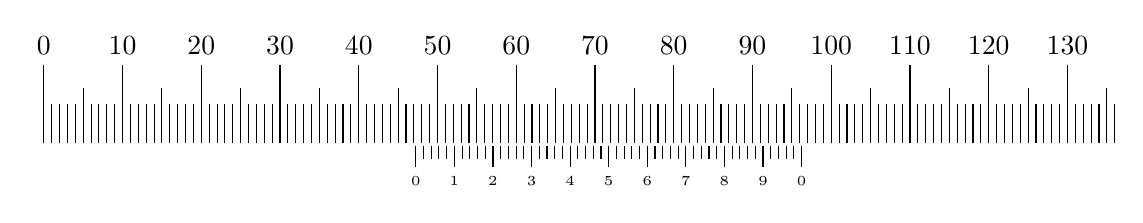
\begin{tikzpicture}

% Escala principal
	\foreach \x in {0.0, 0.1, ..., 13.7}
		\draw (\x,0) -- (\x,0.5);

	\foreach \x in {0, 0.5, ..., 13.5}
		\draw (\x,0) -- (\x,0.7);

	\draw (0,0) -- (0,1) node[anchor=south] {0};
	\foreach \x in {1, 2, ..., 13}
		\draw (\x,0) -- (\x,1) node[anchor=south] {\x0};

% Escala auxiliar
\begin{scope}[xshift=4.724cm]
	\foreach \x in {0.000, 0.098, ..., 4.9}
		\draw (\x,-0.03) -- (\x,-0.2);

	\foreach \x [count=\xi from 0] in {0, 0.490, ..., 4.9}
		\draw (\x,-0.03) -- (\x,-0.3) node[anchor=north] {\tiny \xi};
	
	\draw (4.900,-0.03) -- (4.900,-0.3) node[anchor=north] {\tiny 0};
\end{scope}
\end{tikzpicture}
\caption{Leitura de \np[mm]{47,24}. Note o entre alinhamento a segunda marca após a marca ``2'' na escala auxiliar e a marca da escala principal.\label{Fig:PaquimetroLeitura}}
\end{figure*}

\pagebreak
Na prática, a leitura é bastante simples: 
\begin{enumerate}
	\item Determinamos a leitura da escala principal ---~\np[mm]{47}~---;
	\item Colocamos uma vírgula após o valor dessa leitura ---~\np[mm]{47,}~---;
	\item Verificamos a marca numerada imediatamente à esquerda da marca melhor alinhada e anotamos seu dígito ---~\np[mm]{47,2}~---; \hyphenation{mul-ti-pli-ca-mos}
	\item Finalmente, verificamos a posição da marca melhor alinhada a partir da última numerada ---~nesse caso, a segunda posição~---. Como cada marca da escala auxiliar corresponde a \np[mm]{0,02}, ``multiplicamos'' por dois o ``valor'' da posição e anotamos o resultado ao fim ---~\np[mm]{47,24}~---.
\end{enumerate}
%
Note que nem todas as marcas da escala auxiliar são numeradas, por questão de espaço. Além disso, como a resolução da escala auxiliar é de \np[mm]{0,02}, só é possível obter medidas pares com essa configuração das escalas.

Uma observação importante ao se utilizar equipamentos dotados de escala auxiliar é a realização de medidas que coincidem com as marcas maiores da escala auxiliar. Na Figura~\ref{Fig:PaquimetroLeituraZero}, por exemplo, tempos uma medida em que a marca da escala auxiliar que está alinhada à da escala principal é a denotada pelo número 2. Efetuando a leitura, temos \np[mm]{33,2}. No entanto, temos o último dígito, dado pela ``posição'' da marca alinhada ``multiplicada'' por dois. Se a marca alinhada é a numerada, então a posição é zero. Logo, devemos adicionar um zero ao final da medida: \np[mm]{33,20}. Uma maneira mais simples de interpretar essa questão é verificarmos que \emph{o número de algarismos após a vírgula em uma dada unidade para um instrumento qualquer é sempre o mesmo.} No caso do paquímetro $\np[mm]{1}/50$ dos exemplos acima, o número é sempre de duas casas após a vírgula ao se efetuar medidas em milímetros.
\begin{figure*}
\centering
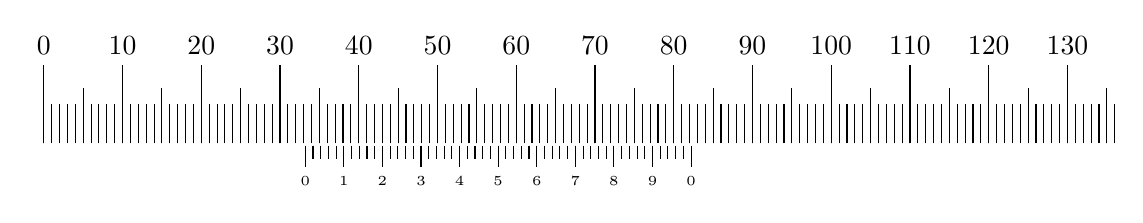
\begin{tikzpicture}

% Escala principal
	\foreach \x in {0.0, 0.1, ..., 13.7}
		\draw (\x,0) -- (\x,0.5);

	\foreach \x in {0, 0.5, ..., 13.5}
		\draw (\x,0) -- (\x,0.7);

	\draw (0,0) -- (0,1) node[anchor=south] {0};
	\foreach \x in {1, 2, ..., 13}
		\draw (\x,0) -- (\x,1) node[anchor=south] {\x0};

% Escala auxiliar
\begin{scope}[xshift=3.320cm]
	\foreach \x in {0.000, 0.098, ..., 4.9}
		\draw (\x,-0.03) -- (\x,-0.2);

	\foreach \x [count=\xi from 0] in {0, 0.490, ..., 4.9}
		\draw (\x,-0.03) -- (\x,-0.3) node[anchor=north] {\tiny \xi};
	
	\draw (4.900,-0.03) -- (4.900,-0.3) node[anchor=north] {\tiny 0};
\end{scope}
\end{tikzpicture}
\caption{Leitura de \np[mm]{33,20}. Note o entre alinhamento a  marca ``2'' na escala auxiliar e a marca da escala principal.\label{Fig:PaquimetroLeituraZero}}
\end{figure*}
%A invenção da escala auxiliar ... \comment{fazer}

%%%%%%%%%%%%%%%%%%%%%%%%%%%%%%%%%%%%%%%%%%%%%%%%%%%%%%%
\paragraph{Paquímetro com divisão de 1 mm em 20 partes}
%%%%%%%%%%%%%%%%%%%%%%%%%%%%%%%%%%%%%%%%%%%%%%%%%%%%%%%

\begin{marginfigure}[3cm]
\centering
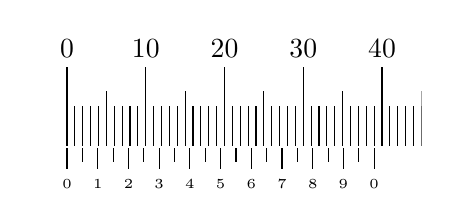
\begin{tikzpicture}

    \clip (-0.5,-0.6) rectangle (4.5,1.5);
    
% Escala principal
	\foreach \x in {0.0, 0.1, ..., 13.7}
		\draw (\x,0) -- (\x,0.5);

	\foreach \x in {0, 0.5, ..., 13.5}
		\draw (\x,0) -- (\x,0.7);

	\draw (0,0) -- (0,1) node[anchor=south] {0};
	\foreach \x in {1, 2, ..., 13}
		\draw (\x,0) -- (\x,1) node[anchor=south] {\x0};

% Escala auxiliar
\begin{scope}[xshift=0.0mm]
	\foreach \x in {0.000, 0.195, ..., 3.89}
		\draw (\x,-0.03) -- (\x,-0.2);

	\foreach \x [count=\xi from 0] in {0, 0.39, ..., 3.89}
		\draw (\x,-0.03) -- (\x,-0.3) node[anchor=north] {\tiny \xi};
	
	\draw (3.9,-0.03) -- (3.9,-0.3) node[anchor=north] {\tiny 0};
\end{scope}
\end{tikzpicture}
\caption{Escala auxiliar 1/20 mm.\label{Fig:Paquimetro20LeituraZero}}
\end{marginfigure}

Para um micrômetro em que dividimos um milímetro em 20 partes o fabricante geralmente escolhe aumentar o espaçamento entre as marcas para facilitar a leitura. O raciocínio, no entanto, é muito similar aos casos anteriores:
\begin{itemize}
	\item Dividimos um milímetro em $n = 20$ partes, obtendo \np[mm]{0.05};
	\item Agora, ao invés elaborar a escala usando $n - 1$ partes, são usadas $2n - 1$ partes, ou seja, a largura entre as marcas da escala auxiliar é de \np[mm]{1,95};
	\item Consequentemente, ao deslocarmos a escala auxiliar para a direita por \np[mm]{0,05}, ocorre o alinhamento entre a primeira marca não numerada da escala auxiliar e a marca de \np[mm]{2,0} na escala principal. Para deslocamentos maiores, temos o alinhamento das marcas subsequentes.
\end{itemize}
%
Novamente, o processo de leitura consiste ---~na prática~--- em:
\begin{itemize}
	\item usar o zero da escala auxiliar para ler a medida da escala principal;
	\item colocar uma vírgula;
	\item verificar qual marca da escala auxiliar tem o melhor alinhamento com uma marca da escala principal. Se for uma das marcas numeradas, temos ``{,}10'', ``{,}20'', ``{,}30'', etc. Se for uma das marcas não numeradas, temos ``{,}15'', ``{,}25'', ``{,}35'', etc.
\end{itemize}

\begin{figure*}
\centering
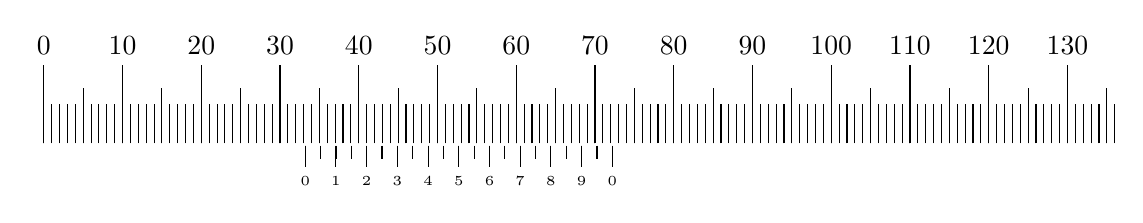
\begin{tikzpicture}

% Escala principal
	\foreach \x in {0.0, 0.1, ..., 13.7}
		\draw (\x,0) -- (\x,0.5);

	\foreach \x in {0, 0.5, ..., 13.5}
		\draw (\x,0) -- (\x,0.7);

	\draw (0,0) -- (0,1) node[anchor=south] {0};
	\foreach \x in {1, 2, ..., 13}
		\draw (\x,0) -- (\x,1) node[anchor=south] {\x0};

% Escala auxiliar
\begin{scope}[xshift=33.20mm]
	\foreach \x in {0.000, 0.195, ..., 3.89}
		\draw (\x,-0.03) -- (\x,-0.2);

	\foreach \x [count=\xi from 0] in {0, 0.39, ..., 3.89}
		\draw (\x,-0.03) -- (\x,-0.3) node[anchor=north] {\tiny \xi};
	
	\draw (3.9,-0.03) -- (3.9,-0.3) node[anchor=north] {\tiny 0};
\end{scope}
\end{tikzpicture}
\caption{A mesma leitura de \np[mm]{33,20} da Figura~\ref{Fig:PaquimetroLeituraZero}, porém em um paquímetro 1/20 mm. Novamente, note o entre alinhamento a  marca ``2'' na escala auxiliar e a marca da escala principal.\label{Fig:Paquimetro20Leitura33mm20}}
\end{figure*}

%%%%%%%%%%%%%%%%%%%%%%%%%%%%%%%%%%%%%%%%%%
\paragraph{Micrômetro com escala auxiliar}
%%%%%%%%%%%%%%%%%%%%%%%%%%%%%%%%%%%%%%%%%%

Micrômetros também podem utilizar escalas auxiliares. Quando elas são utilizadas, não fazemos uma estimativa para obter o último dígito, mas sim uma leitura da escala auxiliar. Nas Figuras~\ref{Fig:MicrometroComEscalaAuxiliar} e~\ref{Fig:DetalheEscalaAuxiliarMicrometro} podemos ver um micrometro dotado de escala auxiliar e o detalhe da escala, respectivamente. Note também que as marcações de milímetros inteiros e meios-milímetros estão ambas na parte inferior da linha central, uma vez que a escala auxiliar toma todo o espaço acima dela. 

\begin{figure}
\centering
\includegraphics[width=0.8\linewidth]{Ilustrations/Micrometro_com_escala_auxiliar.png}
\caption{Micrômetro com escala auxiliar: as marcas à esquerda podem se alinhar com as marcas do tambor (região numerada de 0 a 15 na figura e que pode girar), indicando a leitura apropriada para o último dígito (aquele que é estimado em um micrômetro sem escala auxiliar).\label{Fig:MicrometroComEscalaAuxiliar}}
\end{figure}

\begin{figure}\forceversofloat
\centering
\includegraphics[width=0.75\linewidth]{Ilustrations/Micrometro_com_escala_auxiliar_detalhe.png}
\caption{Detalhe da escala auxiliar de um micrômetro.\label{Fig:DetalheEscalaAuxiliarMicrometro}}
\end{figure}

\pagebreak
Na Figura~\ref{Fig:EscalaMicrometroComEscalaAuxiliar} temos uma representação da escala de um micrômetro com escala auxiliar. A medida da escala principal é feita da mesma maneira que no caso de um micrômetro sem escala auxiliar, isto é, verificamos a marca mais à direita visível. No caso da figura temos \np[mm]{32,5}. Na escala do tambor podemos ver que a linha central passa da marca 19, portanto temos $0{,}19\_\,\text{mm}$, onde `\_' representa o dígito que ainda precisamos determinar através da escala auxiliar. Verificando tal escala, observamos que a primeira linha acima da linha central está alinhada com a marcação do tambor. Logo, o temos $\np[mm]{0,191}$. Finalmente, temos
\begin{align}
	\ell &= \np[mm]{32,5} + \np[mm]{0,191} \\
	&= \np[mm]{32,691}.
\end{align}

\begin{figure}
\centering
\begin{tikzpicture}[scale=1.7]

	\pgfmathsetmacro{\reading}{32.691} % leitura em mm
	
	\pgfmathsetmacro{\decimalpart}{\reading - int(\reading)}  % Extract decimal part
	\pgfmathsetmacro{\scaleddecimal}{\decimalpart * 100}  % Multiply by 100
	\pgfmathsetmacro{\yshift}{mod(\scaleddecimal, 50)}
	\pgfmathsetmacro{\clipsize}{\reading + 10}

	\clip (-0.5,1) rectangle (\clipsize mm,-1);
	
% Escala principal

	\draw (-0.4,0) -- (7,0);
	
	\foreach \x in {0.0, 0.1, ..., 7.0}
		\draw (\x,-0.05) -- (\x,-0.20);

	\foreach \x in {0, 5, ..., 70}
		\draw (\x mm,-0.05) -- (\x mm,-0.3)node[below]{\tiny \x};

	\foreach \x in {0.05, 0.15, ..., 7.0}
		\draw (\x,-0.05) -- (\x,-0.10);
	
	\foreach \y in {1, 3, ..., 9}
		\draw ($(-0.05,\y*0.09)$) -- ($(7,\y*0.09)$);
		
	\foreach \y in {2, 4, ..., 8}
		\draw ($(-0.05,\y*0.09)$) node[left]{\tiny \y} -- ($(7,\y*0.09)$);
		
	\draw (-0.05,0.9) node[left]{\tiny 0} -- (7,0.9);
		
		
% Escala auxiliar
	\begin{scope}[xshift=\reading mm]
		\fill[white] (0,-1) rectangle (1,1);
		\draw[gray] (0,-1) -- (0,1);
		
		\begin{scope}[yshift=-\yshift mm]
			\foreach \y in {0, 1, ...,49}
				\draw (0,\y mm) -- (2 mm,\y mm);

			\foreach \y in {0, 5, ..., 49}{
				%\pgfmathsetmacro{\newy}{int(\y + 10)}
				\draw (0,\y mm) -- (4 mm,\y mm) node[right]{\tiny \y};
			}
			
			\foreach \y in {0, 1, ..., 50}{
				\pgfmathsetmacro{\newy}{int(\y + 50)}
				\draw (0,\newy mm) -- (2 mm,\newy mm);
			}

			\foreach \y in {0, 5, ..., 50}{
				\pgfmathsetmacro{\newy}{int(\y + 50)}
				\draw (0,\newy mm) -- (4 mm,\newy mm) node[right]{\tiny \y};
			}
			
			\foreach \y in {0, 1, ..., 49}{
				\pgfmathsetmacro{\newy}{int(\y - 50)}
				\draw (0,\newy mm) -- (2 mm,\newy mm);
			}
			\foreach \y in {0, 5, ..., 49}{
				\pgfmathsetmacro{\newy}{int(\y - 50)}
				\draw (0,\newy mm) -- (4 mm,\newy mm) node[right]{\tiny \y};
			}
		\end{scope}
	
	\end{scope}
\end{tikzpicture}
\caption{Escala de um micrômetro com escala auxiliar.\label{Fig:EscalaMicrometroComEscalaAuxiliar}}
\end{figure}

%\pagebreak
%%%%%%%%%%%%%%%%%%%%%%%%%%%%%%%%%%%%%%%%%%%%%%%%%%%%%%%%%%%%%%%%%%%%%
\subsection{Unidades e algarismos significativos, notação científica}
\label{Sec:UnidadesAlgSigNotacaoCientifica}
%%%%%%%%%%%%%%%%%%%%%%%%%%%%%%%%%%%%%%%%%%%%%%%%%%%%%%%%%%%%%%%%%%%%%

O número de algarismos significativos de uma medida está ligado à precisão do equipamento utilizado para realizá-la. Devido a isso, se realizarmos uma conversão de unidades, não podemos ter uma alteração no número de algarismos significativos ---~afinal a precisão não aumenta nem diminui~---. Isso nos leva a contemplar as duas seguintes situações:
\begin{enumerate}
\item Realizarmos uma medida e obtemos
\begin{equation}
	\ell = \np[mm]{34,82},
\end{equation}
%
onde o último algarismo foi estimado. Sabemos que temos quatro algarismos significativos e ao expressarmos esta medida em outras unidades, devemos manter o mesmo número de algarismos significativos. Podemos então expressá-la como
\begin{align}
	\ell &= \np[cm]{3,482} \\
	&= \np[dm]{0,3482} \\
	&= \np[m]{0,03482}.
\end{align}
%
Note que os zeros à esquerda não são algarismos significativos. Sua função é exclusivamente a de posicionar a vírgula, dando aos algarismos a ordem de grandeza adequada.

\item Realizamos uma medida de massa obtemos,
\begin{equation}
	m = \np[kg]{11,2},
\end{equation}
%
e desejamos expressá-la em gramas. Efetuando a conversão, poderíamos escrever em um primeiro momento
\begin{equation}
	m = \np[g]{11200}.
\end{equation}
%
Uma medida assim expressa, no entanto, tem cinco algarismos significativos ---~pois o último algarismo anotado é o duvidoso~---, enquanto a medida original tem três.  Portanto, por mais que possamos adicionar zeros ao lado esquerdo sem modificar o número de significativos, não podemos fazê-lo do lado direito. 

Para expressar essa medida com o número adequado de algarismos significativos, podemos utilizar a notação científica. Um número expresso em notação científica tem a forma $a \cdot 10^b$, onde $a$ ---~denominada \emph{mantissa}~--- é um número Real, e $b$ ---~o expoente~--- é um número inteiro. O expoente também é conhecido como \emph{ordem de grandeza}. Em um número expresso dessa forma, somente os algarismos da mantissa são significativos. Os prefixos kilo (k), hecto (h), deci (d), centi (c), mili (m), micro ($\mu$), nano (n), etc., utilizados em unidades de medida são simplesmente formas abreviadas para as notações $\cdot 10^{3}$, $\cdot 10^{2}$, $\cdot 10^{-1}$, $\cdot 10^{-2}$, $\cdot 10^{-3}$, $\cdot 10^{-6}$, $\cdot 10^{-9}$, etc.

Utilizando a notação científica temos então
\begin{equation}
	m = \np[g]{112e2}.
\end{equation}
\end{enumerate}

Portanto, temos as seguintes regras:
\begin{itemize}
	\item Conversões de unidade não alteram a precisão das medidas e por isso não podem alterar o número de algarismos significativos.
	\item Zeros à esquerda não contam como algarismos significativos.
	\item Não podemos adicionar zeros à direita. Se for necessário fazê-lo ao efetuar uma conversão de unidades, devemos utilizar a notação científica.
\end{itemize}

%%%%%%%%%%%%%%%%%%%%%%%%%%%%%%%%%%%%%%%%%%%%%%%%%%%%%%%%%%
\subsection{Operações envolvendo medidas}
%%%%%%%%%%%%%%%%%%%%%%%%%%%%%%%%%%%%%%%%%%%%%%%%%%%%%%%%%%

Lembre-se que em uma medida direta, o algarismo duvidoso está ligado à ideia de que ele seria o algarismo que possivelmente sofreria alterações caso utilizássemos equipamentos mais precisos para realizar as medidas. Isso também se reflete nos valores calculados para medidas indiretas, afinal elas são calculadas a partir de medidas diretas, que têm um algarismo duvidoso. Portanto, ao obtermos uma medida indireta, também devemos denotá-la com o número adequado de algarismos significativos.

Para determiná-los, no entanto, devemos seguir algumas regras para as operações realizadas:
\begin{description}
	\item[Multiplicação e divisão] No caso da multiplicação ou da divisão, devemos limitar o número de algarismos significativos àquele da medida que tiver o menor número.
	
	Para entender a razão dessa regra, podemos fazer a seguinte análise: Tomamos a medida indireta $L$ dada por
\begin{equation}
	L = \ell_1\ell_2\ell_3\dots
\end{equation}
%
onde $\ell_1$, $\ell_2$, $\ell_3$, \dots, são medidas diretas quaisquer. Vamos supor que $\ell_1$ tem $n$ algarismos significativos e que as demais têm mais algarismos significativos que $\ell_1$. Vamos supor ainda que o primeiro dígito (aquele com a maior ordem de grandeza) tem ordem de grandeza $p$, que o duvidoso ordem de grandeza $d$ e que a diferença entre as ordens de grandeza desses dígitos é $s$. Agora fazemos o seguinte
		\begin{enumerate}
			\item Tomamos a ordem de grandeza $d$ do algarismo duvidoso de $\ell_1$ e multiplicamos pelas demais medidas;
			\item Obtemos um valor com uma ordem de grandeza $d'$ qualquer;
			\item Qualquer dígito com uma ordem de grandeza menor que $d'$ é então desprezível se comparado ao dígito com a ordem de grandeza $d$;
			\item Observamos no valor calculado para $L$ que o dígito com a maior ordem de grandeza será $p'$. Esse dígito deve ser $s'$ ordens de grandeza maior que $d'$.
		\end{enumerate}
%
A diferença $s'$ nada mais é do que o número de algarismos significativos da medida $L$. Além disso $s'$ é igual a $s$. Logo, o resultado deve ter o mesmo número de algarismos significativos que a medida $\ell_1$. Portanto, ao multiplicar duas ou mais medidas,
	\begin{itemize}
		\item Determinamos o número de algarismos significativos de cada uma das medidas que compõe o produto/divisão;
		\item Realizamos o produto/divisão;
		\item Ao fim, deixamos o resultado com o mesmo número de algarismos significativos que a medida que tem menos algarismos significativos.
	\end{itemize}
	
	Uma observação importante a se fazer é que se separarmos o cálculo em várias etapas, devemos levar mais algarismos do que o mínimo necessário entre as etapas (pelo menos um a mais). A razão disso é que a contribuição dos dígitos após o último significativo pode se acumular entre as etapas e dar um resultado levemente maior que no caso de os descartarmos. O descarte dos algarismos não-significativos deve ser feito ao final do cálculo.
		
	\textsc{Exemplo}\footnote{Utilizamos a barra para denotar o último algarismo significativo quando escrevemos dígitos além dele.}:
\begin{subequations}\label{Eq:AlgarismosSignificativosMult}
\begin{align}
     \numprint{12,03} \div \numprint{3,6} &= 3,\overline{3}4 = \numprint{3,3} \\
     \numprint{198,633} \times \numprint{3,211} &= 637,\overline{8}1056 = \numprint{637,8}.
\end{align}
\end{subequations}

	\item[Soma e subtração] Para o caso da soma ou subtração, mantemos o número de casas decimais da medida que tem o menor número de casas após a vírgula. 
	
	A razão disso é que se temos uma incerteza em um algarismo qualquer, dígitos à direita serão menores ou da ordem de grandeza da incerteza. Consequentemente, sería inútil expressá-los. Observe que para realizar a soma/subtração, é importante que todas as medidas sejam expressas na mesma unidade e ordem de grandeza.
	
	\textsc{Exemplo:}
\begin{align}
	 \numprint[cm]{12,03} + \numprint[cm]{3,6} &= 15,\overline{6}3~\textrm{cm}\\
		 &= \numprint[cm]{15,6}.
\end{align}

	\item[Constantes] Quando efetuamos uma operação envolvendo uma constante matemática e uma medida, conservamos no resultado o mesmo número de algarismos significativos da medida. 
	
	Nesse caso temos que a constante matemática não tem incerteza nenhuma, então podemos considerá-la com um número infinito de algarismos significativos.
	
	\textsc{Exemplo:}
\begin{align}
	A &= \pi \times (3,66~\textrm{m})^2 \\
	  &= \pi \times (13,\overline{3}956~\textrm{m}^2)\\
	  &= 42,\overline{0}8351855~\textrm{m}^2 \\
	  &= \numprint{42,1}~\textrm{m}^2.
\end{align}

\item[Funções] Quando uma medida é o argumento de uma função, mantemos para o resultado o número de algarismos significativos da medida. 

Uma maneira de entender isso é o fato de que podemos escrever funções como séries de potência\footnote[][-4cm]{Uma série de potência é uma forma de escrever uma função em termos de potências, somas e subtrações. Em geral, tais séries contém um número infinito de termos.

As funções trigonométricas $\sen x$ e $\cos x$, por exemplo, são descritas pelas séries
\begin{align*}
	\sen x = x - \frac{x^3}{3!} + \frac{x^5}{5!} - \frac{x^7}{7!} + \dots \\
	\cos x = 1 - \frac{x^2}{2!} + \frac{x^4}{4!} - \frac{x^6}{6!} + \dots,
\end{align*}
%
onde $x$ é um ângulo expresso em radianos.
} ---~que são basicamente multiplicações, somas e subtrações~---. Dessa forma, podemos verificar que ao tomarmos a medida e realizarmos o produto por ela mesma, devemos ter um resultado com o mesmo número de algarismos significativos para todas as parcelas que serão somadas/subtraídas, sendo que o número de casas após a vírgula fica determinado pelo primeiro termo que não é constante. Assim, ao somarmos, a parcela maior dominará e teremos que o resultado terá o mesmo número de algarismos significativos que o argumento da função\footnote{Isso é útil para podermos truncar a soma da série a um número pequeno de parcelas, afinal não faz sentido calcular parcelas que têm valores menores que a incerteza das parcelas dominantes}.

\textsc{Exemplo:}
\begin{align}
	x &= \ln \numprint{3,555} \\
	&= 1,26\overline{8}355063 \\
	&= 1,268.
\end{align}
\end{description}

%%%%%%%%%%%%%%%%%%%%%%%%%%%%%%%%%%%%%%%%%%%%%%%%%%%%%%%%%%%%%
\subsection{Número de algarismos significativos de uma média}
%%%%%%%%%%%%%%%%%%%%%%%%%%%%%%%%%%%%%%%%%%%%%%%%%%%%%%%%%%%%%

Ao realizarmos uma média, somamos $n$ medidas e então dividimos por $n$. Através das regras apresentadas acima, ao somarmos, temos um possível aumento do número de algarismos significativos. Como $n$ é uma contagem e não uma medida, ao realizarmos a divsião, obtemos um valor \emph{com mais algarismos significativos que as parcelas da soma}. Por exemplo, se temos as medidas
\begin{align}
	\ell_1 &= \np[cm]{32,5} \\
	\ell_2 &= \np[cm]{33,8} \\
	\ell_3 &= \np[cm]{37,3},
\end{align}
%
ao somarmos obtemos
\begin{equation}
	\ell_S = \np[cm]{103,6}.
\end{equation}
%
Finalmente, ao realizarmos a divisão, temos
\begin{equation}
	\mean{\ell} = \np[cm]{34,55}.
\end{equation}

Embora esse resultado pareça estranho, de acordo com as regras de algarismos significativos, ele faz sentido de um ponto de vista estatístico, onde é possível mostrar que o erro da média é inversamente proporcional à raiz quadrada do número de medidas. Na verdade, os algarismos significativos são apenas uma regra simples para tratar as medidas sem que seja necessário utilizar uma matemática mais robusta, porém trabalhosa.

%%%%%%%%%%%%%%%%%%%%%%%%%%%%%
\subsection{Arredondamento}
%%%%%%%%%%%%%%%%%%%%%%%%%%%%%

Nos exemplos da seção anterior, usamos uma barra para denotar o último algarismo significativo antes de descartar os algarismos excedentes. Sempre que os descartarmos, devemos fazê-lo observando os critérios de arredondamento.

Quando obtemos resultados do tipo
\begin{equation}
     \ell = 134,\overline{3}9487,
\end{equation}
%
precisamos fazer um \emph{arredondamento}. No exemplo acima, vemos que 134,4 é um número mais próximo do resultado do que 134,3. Portanto, adotamos as seguintes regras ao realizarmos o arredondamento:
\begin{enumerate}
     \item Se o algarismo seguinte ao duvidoso for menor que 5, simplesmente descartamos os algarismos excedentes.
     \item Se o algarismo seguinte ao duvidoso for maior ou igual a 5, aumentamos o duvidoso de uma unidade e descartamos os demais.
\end{enumerate}
%
Esse critério de arredondamento não é único. Em algumas situações se utiliza uma regra específica para o caso de o algarismo seguinte ao duvidoso ser 5: analisa-se o algarismo seguinte a esse e caso ele for par, se arredonda para cima e caso for ímpar, para baixo.

%%%%%%%%%%%%%%%%%%%%
\section{Exercícios}
%%%%%%%%%%%%%%%%%%%%

%%%%%%%%%%%%%%%%%%%%%%%%%%%%%
\begin{question}[type={exam}]
Determine o resultado das somas e subtrações abaixo com o número adequado de algarismos significativos.
\begin{multicols}{2}
\begin{enumerate}
\item $12{,}45\ \text{cm} + 3{,}2\ \text{cm}$
\item $0{,}0045\ \text{m} - 0{,}003\ \text{m}$
\item $5{,}67\ \text{kg} + 2{,}1\ \text{kg}$
\item $18{,}0\ \text{mL} - 0{,}45\ \text{mL}$
\item $3{,}456\ \text{m} + 0{,}12\ \text{m}$
\item $7{,}89\ \text{g} - 2{,}3\ \text{g}$
\item $0{,}0056\ \text{L} + 0{,}002\ \text{L}$
\item $9{,}0\ \text{cm} - 4{,}56\ \text{cm}$
\item $1{,}234\ \text{m} + 2{,}1\ \text{m}$
\item $6{,}78\ \text{kg} - 1{,}234\ \text{kg}$
\item $0{,}00345\ \text{m} + 0{,}0007\ \text{m}$
\item $4{,}56\ \text{cm} - 1{,}2\ \text{cm}$
\item $2{,}789\ \text{g} + 0{,}34\ \text{g}$
\item $10{,}0\ \text{mL} - 9{,}876\ \text{mL}$
\item $0{,}00045\ \text{kg} + 0{,}00012\ \text{kg}$
\item $3{,}45\ \text{m} - 1{,}234\ \text{m}$
\item $7{,}890\ \text{cm} + 0{,}12\ \text{cm}$
\item $0{,}0000034\ \text{m} + 0{,}00000056\ \text{m}$
\item $6{,}78 \cdot 10^5\ \text{g} + 1{,}2 \cdot 10^4\ \text{g}$
\item $9{,}0 \cdot 10^{-3}\ \text{m} - 4{,}56 \cdot 10^{-4}\ \text{m}$
\end{enumerate}
\end{multicols}
\end{question}

%%%%%%%%%%%%%%%%%%%%%%%%%%%%%
\begin{question}[type={exam}]
Determine o resultado das multiplicações e divisões abaixo com o número adequado de algarismos significativos.
\begin{multicols}{2}
\begin{enumerate}
\item $3{,}2\,\text{m} \times 2{,}1\,\text{m}$
\item $6{,}40\,\text{s} \div 2{,}0\,\text{s}$
\item $8{,}55\,\text{kg} \times 3{,}1$
\item $9{,}0\,\text{m} \div 1{,}5\,\text{s}$
\item $7{,}345\,\text{m} \div 2{,}1$
\item $2{,}00\,\text{m} \times 3{,}0\,\text{m}$
\item $1{,}75\,\text{m/s}^2 \div 2{,}5$
\item $4{,}32\,\text{N} \times 0{,}25$
\item $5{,}10\,\text{m/s} \div 2{,}00\,\text{s}$
\item $7{,}0\,\text{kg} \times 1{,}50\,\text{m/s}^2$
\item $3{,}00\,\text{m} \div 4{,}0$
\item $6{,}78\,\text{cm} \div 2{,}1\,\text{s}$
\item $50{,}25\,\text{kg} \times 2{,}0\,\text{m/s}^2$
\item $9{,}60\,\text{m} \div 3{,}2\,\text{m}$
\item $2{,}20\,\text{L} \times 1{,}50$
\item $3{,}45 \cdot 10^5\,\text{m} \div 1{,}5 \cdot 10^2\,\text{s}$
\item $1{,}67 \cdot 10^{-2}\,\text{kg} \times 6{,}40 \cdot 10^{3}\,\text{m}^2$
\item $9{,}1 \cdot 10^{-31}\,\text{kg} \div 3{,}0 \cdot 10^{8}\,\text{m/s}$
\item $3{,}00 \cdot 10^8\,\text{m/s} \times 2{,}0 \cdot 10^{-6}\,\text{s}$
\item $5{,}523 \cdot 10^2\,\text{kg} \div 2{,}2 \cdot 10^{-1}\,\text{m}^3$
\end{enumerate}
\end{multicols}
\end{question}

%%%%%%%%%%%%%%%%%%%%%%%%%%%%%
\begin{question}[type={exam}]
Determine o resultado das funções abaixo com o número adequado de algarismos significativos. Nos casos em que possa haver alguma ambiguidade, as medidas foram postas entre parêntesis.
\begin{multicols}{2}
\begin{enumerate}
\item $\sin(10{,}48)$
\item $\cos(5{,}25)$
\item $\tan(0{,}78)$
\item $\log(100{,}0)$
\item $\ln(2{,}71)$
\item $\mathrm{e}^{1{,}23}$
\item $\sqrt{3{,}60\,\text{m}}$
\item $(5{,}21)^2$
\item $10^{(3{,}4)}$
\item $(0{,}4500)^{-1}$
\end{enumerate}
\end{multicols}
\end{question}

%%%%%%%%%%%%%%%%%%%%%%%%%%%%%
\begin{question}[type={exam}]
Determine o resultado das multiplicações e divisões por constantes abaixo com o número adequado de algarismos significativos.
\begin{multicols}{2}
\begin{enumerate}
\item $5{,}0\,\text{m} \times 2$
\item $12{,}4\,\text{s} \div 4$
\item $3{,}5\,\text{kg} \times \pi$
\item $7{,}00\,\text{m} \div \pi$
\item $2{,}0\,\text{L} \times \mathrm{e}$
\item $10{,}0\,\text{J} \div \mathrm{e}$
\item $9{,}81\,\text{m/s}^2 \times 3$
\item $897{,}0 \, \text{J/kg}^\circ\text{C} \div 2$
\item $15{,}0\,\text{cm} \div 5$
\item $4{,}50\,\text{m} \times \dfrac{\pi}{2}$
\end{enumerate}
\end{multicols}
\end{question}

%%%%%%%%%%%%%%%%%%%%%%%%%%%%%
\begin{question}[type={exam}]
Determine o resultado das operações abaixo com o número adequado de algarismos significativos.
\begin{multicols}{2}
\begin{enumerate}
\item $\sqrt{(2{,}5\,\text{m})^2 + (4{,}0\,\text{m})^2}$
\item $(5{,}0\,\text{s} + 2{,}75\,\text{s}) \times 3$
\item $\dfrac{10{,}0\,\text{kg} \times 9{,}81\,\text{m/s}^2}{\pi}$
\item $\mathrm{e}^{0{,}50} \times 2{,}00\,\text{J}$
\item $\dfrac{3{,}5\,\text{L}}{\ln(2,00)}$
\item $(4{,}00\,\text{m} - 2{,}25\,\text{m}) \times \pi$
\item $6{,}0\,\text{m/s} \times \cos(60,0^\circ)$
\item $5{,}0\,\text{kg} \times 9{,}81\,\text{m/s}^2 \times \sin(\pi/6)$
\item $\dfrac{12{,}0\,\text{cm} \times \pi}{4}$
\item $2{,}50\,\text{L} \div \mathrm{e}^{1{,}2}$
\item $\ln(6,8) \times 1{,}01\,\text{s}$
\item $10^{2{,}0} \div 4$
\item $3{,}00\,\text{m} + \sqrt{2{,}25\,\text{m}^2}$
\item $\dfrac{(6{,}0\,\text{kg})^2}{2 \times 3{,}0\,\text{kg}}$
\item $2{,}0\,\text{m} \times \dfrac{\pi}{3} + 1{,}5\,\text{m}$
\item $\dfrac{1}{\sqrt{0{,}25\,\text{s}^2}}$
\item $(5{,}25\,\text{m/s}) \times \mathrm{e}^{-0{,}5}$
\item $10{,}0\,\text{m} - \dfrac{3{,}00\,\text{m}}{\pi}$
\item $\dfrac{4{,}0\,\text{m}}{2{,}0} + \dfrac{\sqrt{9{,}0\,\text{m}^2}}{1{,}01\,\text{s}}$
\item $3{,}0\,\text{kg} \times \left( 9{,}81\,\text{m/s}^2 \times \cos(30^\circ) \right)$
\end{enumerate}

\end{multicols}
\end{question}

%%%%%%%%%%%%%%%%%%%%%%%%%%%%%
\begin{question}[type={exam}]
Faça a leitura das medidas mostradas nas figuras abaixo.
\end{question}

\begin{figure*}
\centering
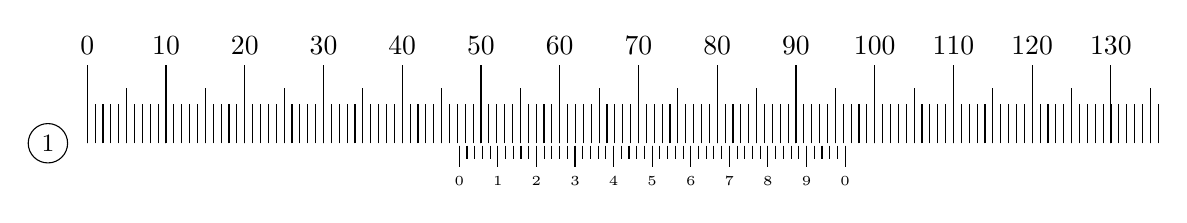
\begin{tikzpicture}

\node[circle, draw, minimum size=5mm, inner sep=0pt] (N) at (-0.5,0) {\small 1};

% Escala principal
	\foreach \x in {0.0, 0.1, ..., 13.7}
		\draw (\x,0) -- (\x,0.5);

	\foreach \x in {0, 0.5, ..., 13.5}
		\draw (\x,0) -- (\x,0.7);

	\draw (0,0) -- (0,1) node[anchor=south] {0};
	\foreach \x in {1, 2, ..., 13}
		\draw (\x,0) -- (\x,1) node[anchor=south] {\x0};

% Escala auxiliar
\begin{scope}[xshift=47.24mm]
	\foreach \x in {0.000, 0.098, ..., 4.9}
		\draw (\x,-0.03) -- (\x,-0.2);

	\foreach \x [count=\xi from 0] in {0, 0.490, ..., 4.9}
		\draw (\x,-0.03) -- (\x,-0.3) node[anchor=north] {\tiny \xi};
	
	\draw (4.900,-0.03) -- (4.900,-0.3) node[anchor=north] {\tiny 0};
\end{scope}
\end{tikzpicture}
\end{figure*}

\begin{figure*}
\centering
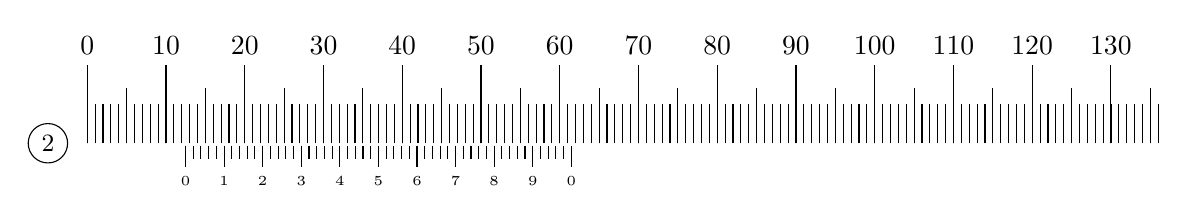
\begin{tikzpicture}

\node[circle, draw, minimum size=5mm, inner sep=0pt] (N) at (-0.5,0) {\small 2};

% Escala principal
	\foreach \x in {0.0, 0.1, ..., 13.7}
		\draw (\x,0) -- (\x,0.5);

	\foreach \x in {0, 0.5, ..., 13.5}
		\draw (\x,0) -- (\x,0.7);

	\draw (0,0) -- (0,1) node[anchor=south] {0};
	\foreach \x in {1, 2, ..., 13}
		\draw (\x,0) -- (\x,1) node[anchor=south] {\x0};

% Escala auxiliar
\begin{scope}[xshift=12.47 mm]
	\foreach \x in {0.000, 0.098, ..., 4.9}
		\draw (\x,-0.03) -- (\x,-0.2);

	\foreach \x [count=\xi from 0] in {0, 0.490, ..., 4.9}
		\draw (\x,-0.03) -- (\x,-0.3) node[anchor=north] {\tiny \xi};
	
	\draw (4.900,-0.03) -- (4.900,-0.3) node[anchor=north] {\tiny 0};
\end{scope}
\end{tikzpicture}
\end{figure*}

\begin{figure*}
\centering
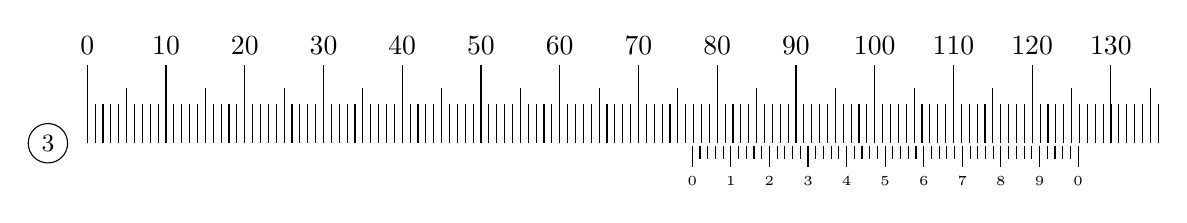
\begin{tikzpicture}

\node[circle, draw, minimum size=5mm, inner sep=0pt] (N) at (-0.5,0) {\small 3};

% Escala principal
	\foreach \x in {0.0, 0.1, ..., 13.7}
		\draw (\x,0) -- (\x,0.5);

	\foreach \x in {0, 0.5, ..., 13.5}
		\draw (\x,0) -- (\x,0.7);

	\draw (0,0) -- (0,1) node[anchor=south] {0};
	\foreach \x in {1, 2, ..., 13}
		\draw (\x,0) -- (\x,1) node[anchor=south] {\x0};

% Escala auxiliar
\begin{scope}[xshift=76.83mm]
	\foreach \x in {0.000, 0.098, ..., 4.9}
		\draw (\x,-0.03) -- (\x,-0.2);

	\foreach \x [count=\xi from 0] in {0, 0.490, ..., 4.9}
		\draw (\x,-0.03) -- (\x,-0.3) node[anchor=north] {\tiny \xi};
	
	\draw (4.900,-0.03) -- (4.900,-0.3) node[anchor=north] {\tiny 0};
\end{scope}
\end{tikzpicture}
\end{figure*}

\begin{figure*}
\centering
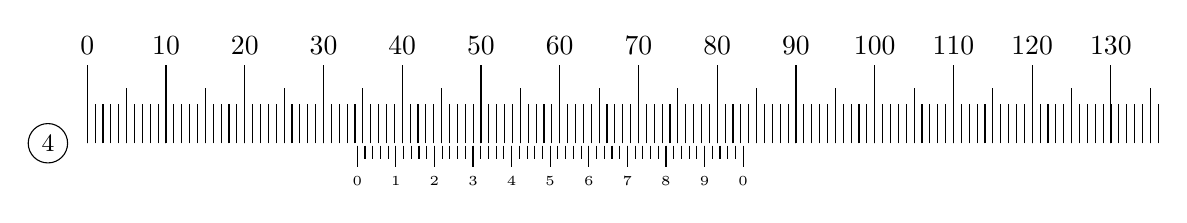
\begin{tikzpicture}

\node[circle, draw, minimum size=5mm, inner sep=0pt] (N) at (-0.5,0) {\small 4};

% Escala principal
	\foreach \x in {0.0, 0.1, ..., 13.7}
		\draw (\x,0) -- (\x,0.5);

	\foreach \x in {0, 0.5, ..., 13.5}
		\draw (\x,0) -- (\x,0.7);

	\draw (0,0) -- (0,1) node[anchor=south] {0};
	\foreach \x in {1, 2, ..., 13}
		\draw (\x,0) -- (\x,1) node[anchor=south] {\x0};

% Escala auxiliar
\begin{scope}[xshift=34.29mm]
	\foreach \x in {0.000, 0.098, ..., 4.9}
		\draw (\x,-0.03) -- (\x,-0.2);

	\foreach \x [count=\xi from 0] in {0, 0.490, ..., 4.9}
		\draw (\x,-0.03) -- (\x,-0.3) node[anchor=north] {\tiny \xi};
	
	\draw (4.900,-0.03) -- (4.900,-0.3) node[anchor=north] {\tiny 0};
\end{scope}
\end{tikzpicture}
\end{figure*}

\begin{figure*}
\centering
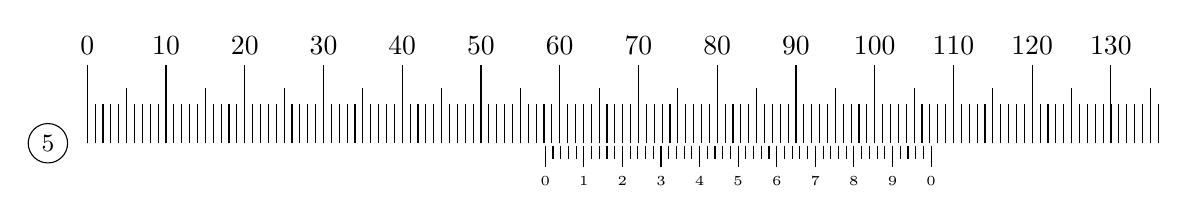
\begin{tikzpicture}

\node[circle, draw, minimum size=5mm, inner sep=0pt] (N) at (-0.5,0) {\small 5};

% Escala principal
	\foreach \x in {0.0, 0.1, ..., 13.7}
		\draw (\x,0) -- (\x,0.5);

	\foreach \x in {0, 0.5, ..., 13.5}
		\draw (\x,0) -- (\x,0.7);

	\draw (0,0) -- (0,1) node[anchor=south] {0};
	\foreach \x in {1, 2, ..., 13}
		\draw (\x,0) -- (\x,1) node[anchor=south] {\x0};

% Escala auxiliar
\begin{scope}[xshift=58.16mm]
	\foreach \x in {0.000, 0.098, ..., 4.9}
		\draw (\x,-0.03) -- (\x,-0.2);

	\foreach \x [count=\xi from 0] in {0, 0.490, ..., 4.9}
		\draw (\x,-0.03) -- (\x,-0.3) node[anchor=north] {\tiny \xi};
	
	\draw (4.900,-0.03) -- (4.900,-0.3) node[anchor=north] {\tiny 0};
\end{scope}
\end{tikzpicture}
\end{figure*}

\begin{figure*}
\centering
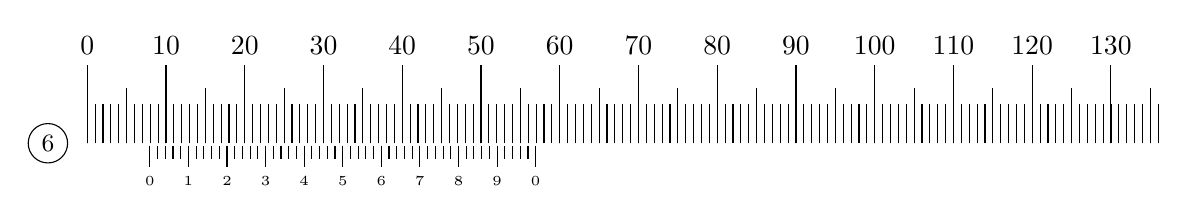
\begin{tikzpicture}

\node[circle, draw, minimum size=5mm, inner sep=0pt] (N) at (-0.5,0) {\small 6};

% Escala principal
	\foreach \x in {0.0, 0.1, ..., 13.7}
		\draw (\x,0) -- (\x,0.5);

	\foreach \x in {0, 0.5, ..., 13.5}
		\draw (\x,0) -- (\x,0.7);

	\draw (0,0) -- (0,1) node[anchor=south] {0};
	\foreach \x in {1, 2, ..., 13}
		\draw (\x,0) -- (\x,1) node[anchor=south] {\x0};

% Escala auxiliar
\begin{scope}[xshift=7.94mm]
	\foreach \x in {0.000, 0.098, ..., 4.9}
		\draw (\x,-0.03) -- (\x,-0.2);

	\foreach \x [count=\xi from 0] in {0, 0.490, ..., 4.9}
		\draw (\x,-0.03) -- (\x,-0.3) node[anchor=north] {\tiny \xi};
	
	\draw (4.900,-0.03) -- (4.900,-0.3) node[anchor=north] {\tiny 0};
\end{scope}
\end{tikzpicture}
\end{figure*}

\begin{figure*}
\centering
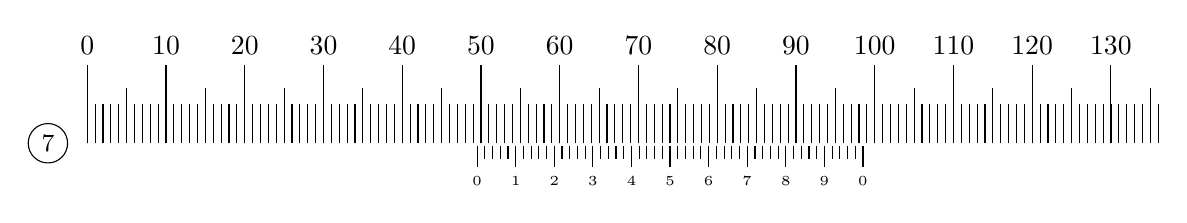
\begin{tikzpicture}

\node[circle, draw, minimum size=5mm, inner sep=0pt] (N) at (-0.5,0) {\small 7};

% Escala principal
	\foreach \x in {0.0, 0.1, ..., 13.7}
		\draw (\x,0) -- (\x,0.5);

	\foreach \x in {0, 0.5, ..., 13.5}
		\draw (\x,0) -- (\x,0.7);

	\draw (0,0) -- (0,1) node[anchor=south] {0};
	\foreach \x in {1, 2, ..., 13}
		\draw (\x,0) -- (\x,1) node[anchor=south] {\x0};

% Escala auxiliar
\begin{scope}[xshift=49.51mm]
	\foreach \x in {0.000, 0.098, ..., 4.9}
		\draw (\x,-0.03) -- (\x,-0.2);

	\foreach \x [count=\xi from 0] in {0, 0.490, ..., 4.9}
		\draw (\x,-0.03) -- (\x,-0.3) node[anchor=north] {\tiny \xi};
	
	\draw (4.900,-0.03) -- (4.900,-0.3) node[anchor=north] {\tiny 0};
\end{scope}
\end{tikzpicture}
\end{figure*}

\begin{figure*}
\centering
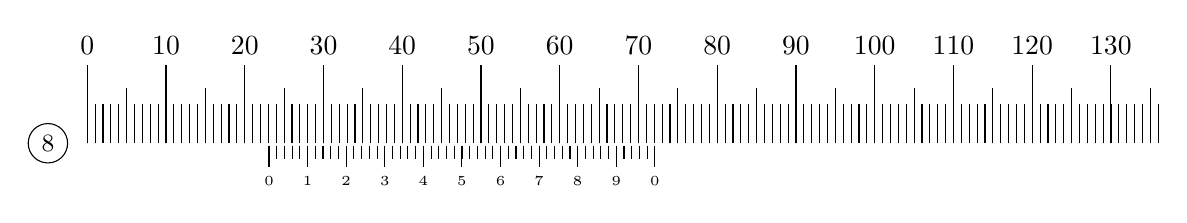
\begin{tikzpicture}

\node[circle, draw, minimum size=5mm, inner sep=0pt] (N) at (-0.5,0) {\small 8};

% Escala principal
	\foreach \x in {0.0, 0.1, ..., 13.7}
		\draw (\x,0) -- (\x,0.5);

	\foreach \x in {0, 0.5, ..., 13.5}
		\draw (\x,0) -- (\x,0.7);

	\draw (0,0) -- (0,1) node[anchor=south] {0};
	\foreach \x in {1, 2, ..., 13}
		\draw (\x,0) -- (\x,1) node[anchor=south] {\x0};

% Escala auxiliar
\begin{scope}[xshift=23.08mm]
	\foreach \x in {0.000, 0.098, ..., 4.9}
		\draw (\x,-0.03) -- (\x,-0.2);

	\foreach \x [count=\xi from 0] in {0, 0.490, ..., 4.9}
		\draw (\x,-0.03) -- (\x,-0.3) node[anchor=north] {\tiny \xi};
	
	\draw (4.900,-0.03) -- (4.900,-0.3) node[anchor=north] {\tiny 0};
\end{scope}
\end{tikzpicture}
\end{figure*}

\begin{figure*}
\centering
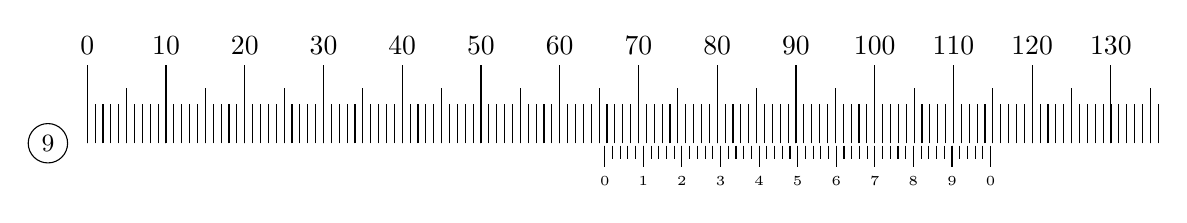
\begin{tikzpicture}

\node[circle, draw, minimum size=5mm, inner sep=0pt] (N) at (-0.5,0) {\small 9};

% Escala principal
	\foreach \x in {0.0, 0.1, ..., 13.7}
		\draw (\x,0) -- (\x,0.5);

	\foreach \x in {0, 0.5, ..., 13.5}
		\draw (\x,0) -- (\x,0.7);

	\draw (0,0) -- (0,1) node[anchor=south] {0};
	\foreach \x in {1, 2, ..., 13}
		\draw (\x,0) -- (\x,1) node[anchor=south] {\x0};

% Escala auxiliar
\begin{scope}[xshift=65.72mm]
	\foreach \x in {0.000, 0.098, ..., 4.9}
		\draw (\x,-0.03) -- (\x,-0.2);

	\foreach \x [count=\xi from 0] in {0, 0.490, ..., 4.9}
		\draw (\x,-0.03) -- (\x,-0.3) node[anchor=north] {\tiny \xi};
	
	\draw (4.900,-0.03) -- (4.900,-0.3) node[anchor=north] {\tiny 0};
\end{scope}
\end{tikzpicture}
\end{figure*}

\begin{figure*}
\centering
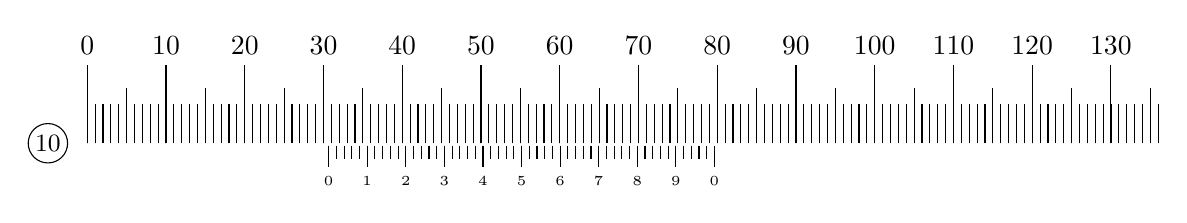
\begin{tikzpicture}

\node[circle, draw, minimum size=5mm, inner sep=0pt] (N) at (-0.5,0) {\small 10};

% Escala principal
	\foreach \x in {0.0, 0.1, ..., 13.7}
		\draw (\x,0) -- (\x,0.5);

	\foreach \x in {0, 0.5, ..., 13.5}
		\draw (\x,0) -- (\x,0.7);

	\draw (0,0) -- (0,1) node[anchor=south] {0};
	\foreach \x in {1, 2, ..., 13}
		\draw (\x,0) -- (\x,1) node[anchor=south] {\x0};

% Escala auxiliar
\begin{scope}[xshift=30.65mm]
	\foreach \x in {0.000, 0.098, ..., 4.9}
		\draw (\x,-0.03) -- (\x,-0.2);

	\foreach \x [count=\xi from 0] in {0, 0.490, ..., 4.9}
		\draw (\x,-0.03) -- (\x,-0.3) node[anchor=north] {\tiny \xi};
	
	\draw (4.900,-0.03) -- (4.900,-0.3) node[anchor=north] {\tiny 0};
\end{scope}
\end{tikzpicture}
\end{figure*}

\begin{figure*}
\centering
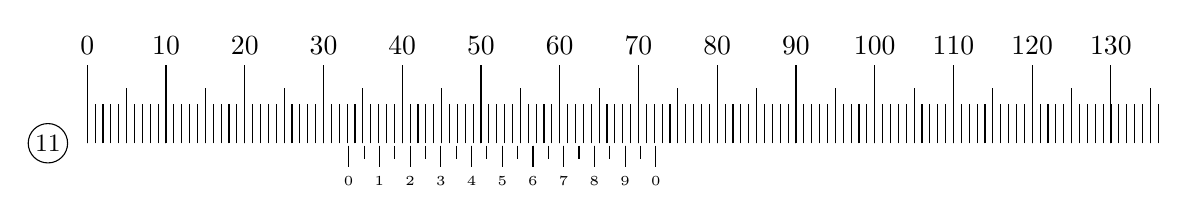
\begin{tikzpicture}

\node[circle, draw, minimum size=5mm, inner sep=0pt] (N) at (-0.5,0) {\small 11};

% Escala principal
	\foreach \x in {0.0, 0.1, ..., 13.7}
		\draw (\x,0) -- (\x,0.5);

	\foreach \x in {0, 0.5, ..., 13.5}
		\draw (\x,0) -- (\x,0.7);

	\draw (0,0) -- (0,1) node[anchor=south] {0};
	\foreach \x in {1, 2, ..., 13}
		\draw (\x,0) -- (\x,1) node[anchor=south] {\x0};

% Escala auxiliar
\begin{scope}[xshift=33.20mm]
	\foreach \x in {0.000, 0.195, ..., 3.89}
		\draw (\x,-0.03) -- (\x,-0.2);

	\foreach \x [count=\xi from 0] in {0, 0.39, ..., 3.89}
		\draw (\x,-0.03) -- (\x,-0.3) node[anchor=north] {\tiny \xi};
	
	\draw (3.9,-0.03) -- (3.9,-0.3) node[anchor=north] {\tiny 0};
\end{scope}
\end{tikzpicture}
\end{figure*}

\begin{figure*}
\centering
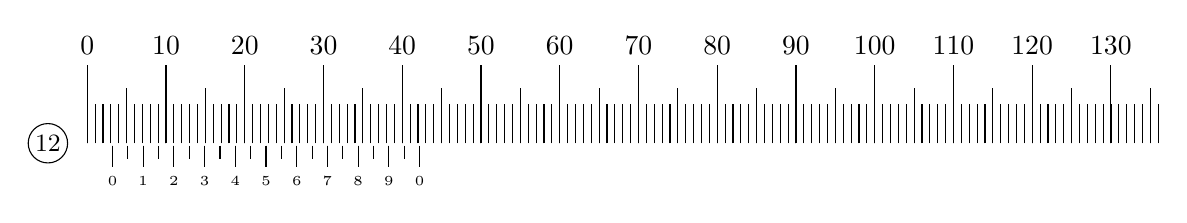
\begin{tikzpicture}

\node[circle, draw, minimum size=5mm, inner sep=0pt] (N) at (-0.5,0) {\small 12};

% Escala principal
	\foreach \x in {0.0, 0.1, ..., 13.7}
		\draw (\x,0) -- (\x,0.5);

	\foreach \x in {0, 0.5, ..., 13.5}
		\draw (\x,0) -- (\x,0.7);

	\draw (0,0) -- (0,1) node[anchor=south] {0};
	\foreach \x in {1, 2, ..., 13}
		\draw (\x,0) -- (\x,1) node[anchor=south] {\x0};

% Escala auxiliar
\begin{scope}[xshift=3.20mm]
	\foreach \x in {0.000, 0.195, ..., 3.89}
		\draw (\x,-0.03) -- (\x,-0.2);

	\foreach \x [count=\xi from 0] in {0, 0.39, ..., 3.89}
		\draw (\x,-0.03) -- (\x,-0.3) node[anchor=north] {\tiny \xi};
	
	\draw (3.9,-0.03) -- (3.9,-0.3) node[anchor=north] {\tiny 0};
\end{scope}
\end{tikzpicture}
\end{figure*}

\begin{figure*}
\centering
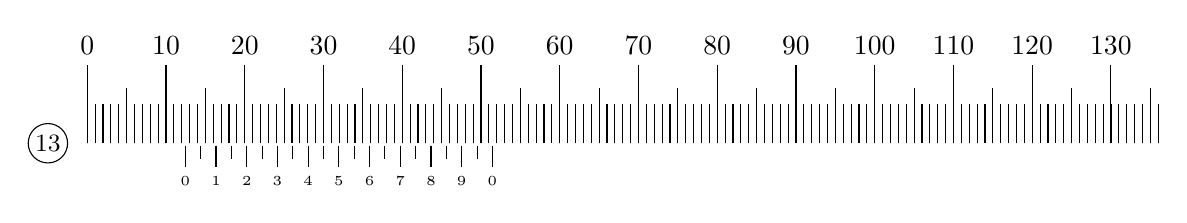
\begin{tikzpicture}

\node[circle, draw, minimum size=5mm, inner sep=0pt] (N) at (-0.5,0) {\small 13};

% Escala principal
	\foreach \x in {0.0, 0.1, ..., 13.7}
		\draw (\x,0) -- (\x,0.5);

	\foreach \x in {0, 0.5, ..., 13.5}
		\draw (\x,0) -- (\x,0.7);

	\draw (0,0) -- (0,1) node[anchor=south] {0};
	\foreach \x in {1, 2, ..., 13}
		\draw (\x,0) -- (\x,1) node[anchor=south] {\x0};

% Escala auxiliar
\begin{scope}[xshift=12.45mm]
	\foreach \x in {0.000, 0.195, ..., 3.89}
		\draw (\x,-0.03) -- (\x,-0.2);

	\foreach \x [count=\xi from 0] in {0, 0.39, ..., 3.89}
		\draw (\x,-0.03) -- (\x,-0.3) node[anchor=north] {\tiny \xi};
	
	\draw (3.9,-0.03) -- (3.9,-0.3) node[anchor=north] {\tiny 0};
\end{scope}
\end{tikzpicture}
\end{figure*}

\begin{figure*}
\centering
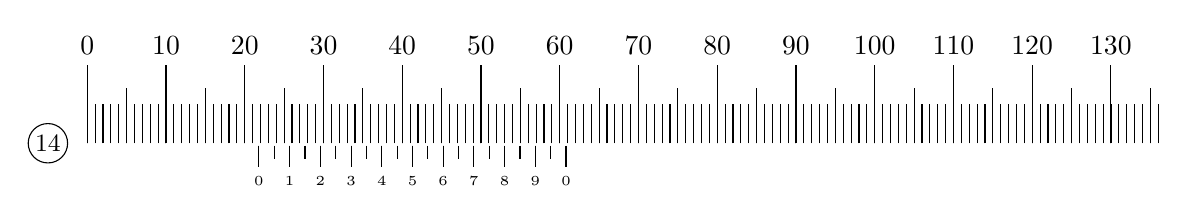
\begin{tikzpicture}

\node[circle, draw, minimum size=5mm, inner sep=0pt] (N) at (-0.5,0) {\small 14};

% Escala principal
	\foreach \x in {0.0, 0.1, ..., 13.7}
		\draw (\x,0) -- (\x,0.5);

	\foreach \x in {0, 0.5, ..., 13.5}
		\draw (\x,0) -- (\x,0.7);

	\draw (0,0) -- (0,1) node[anchor=south] {0};
	\foreach \x in {1, 2, ..., 13}
		\draw (\x,0) -- (\x,1) node[anchor=south] {\x0};

% Escala auxiliar
\begin{scope}[xshift=21.80mm]
	\foreach \x in {0.000, 0.195, ..., 3.89}
		\draw (\x,-0.03) -- (\x,-0.2);

	\foreach \x [count=\xi from 0] in {0, 0.39, ..., 3.89}
		\draw (\x,-0.03) -- (\x,-0.3) node[anchor=north] {\tiny \xi};
	
	\draw (3.9,-0.03) -- (3.9,-0.3) node[anchor=north] {\tiny 0};
\end{scope}
\end{tikzpicture}
\end{figure*}

\begin{figure*}
\centering
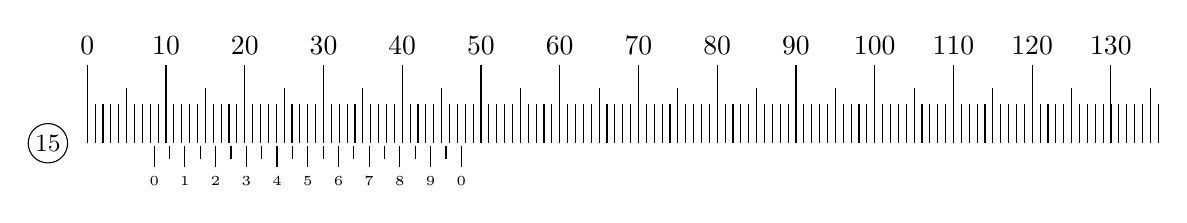
\begin{tikzpicture}

\node[circle, draw, minimum size=5mm, inner sep=0pt] (N) at (-0.5,0) {\small 15};

% Escala principal
	\foreach \x in {0.0, 0.1, ..., 13.7}
		\draw (\x,0) -- (\x,0.5);

	\foreach \x in {0, 0.5, ..., 13.5}
		\draw (\x,0) -- (\x,0.7);

	\draw (0,0) -- (0,1) node[anchor=south] {0};
	\foreach \x in {1, 2, ..., 13}
		\draw (\x,0) -- (\x,1) node[anchor=south] {\x0};

% Escala auxiliar
\begin{scope}[xshift=8.50mm]
	\foreach \x in {0.000, 0.195, ..., 3.89}
		\draw (\x,-0.03) -- (\x,-0.2);

	\foreach \x [count=\xi from 0] in {0, 0.39, ..., 3.89}
		\draw (\x,-0.03) -- (\x,-0.3) node[anchor=north] {\tiny \xi};
	
	\draw (3.9,-0.03) -- (3.9,-0.3) node[anchor=north] {\tiny 0};
\end{scope}
\end{tikzpicture}
\end{figure*}

\begin{figure*}
\centering
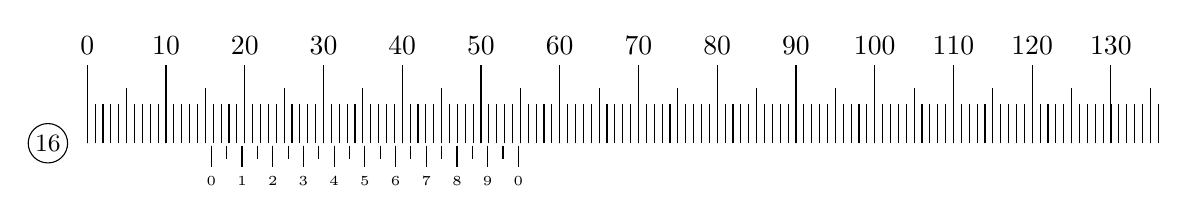
\begin{tikzpicture}

\node[circle, draw, minimum size=5mm, inner sep=0pt] (N) at (-0.5,0) {\small 16};

% Escala principal
	\foreach \x in {0.0, 0.1, ..., 13.7}
		\draw (\x,0) -- (\x,0.5);

	\foreach \x in {0, 0.5, ..., 13.5}
		\draw (\x,0) -- (\x,0.7);

	\draw (0,0) -- (0,1) node[anchor=south] {0};
	\foreach \x in {1, 2, ..., 13}
		\draw (\x,0) -- (\x,1) node[anchor=south] {\x0};

% Escala auxiliar
\begin{scope}[xshift=15.75mm]
	\foreach \x in {0.000, 0.195, ..., 3.89}
		\draw (\x,-0.03) -- (\x,-0.2);

	\foreach \x [count=\xi from 0] in {0, 0.39, ..., 3.89}
		\draw (\x,-0.03) -- (\x,-0.3) node[anchor=north] {\tiny \xi};
	
	\draw (3.9,-0.03) -- (3.9,-0.3) node[anchor=north] {\tiny 0};
\end{scope}
\end{tikzpicture}
\end{figure*}

\begin{figure*}
\centering
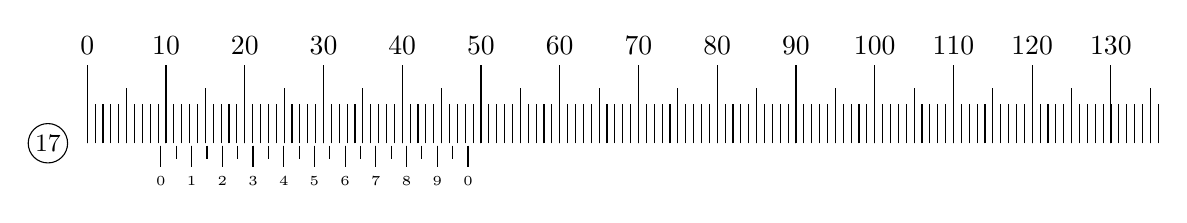
\begin{tikzpicture}

\node[circle, draw, minimum size=5mm, inner sep=0pt] (N) at (-0.5,0) {\small 17};

% Escala principal
	\foreach \x in {0.0, 0.1, ..., 13.7}
		\draw (\x,0) -- (\x,0.5);

	\foreach \x in {0, 0.5, ..., 13.5}
		\draw (\x,0) -- (\x,0.7);

	\draw (0,0) -- (0,1) node[anchor=south] {0};
	\foreach \x in {1, 2, ..., 13}
		\draw (\x,0) -- (\x,1) node[anchor=south] {\x0};

% Escala auxiliar
\begin{scope}[xshift=9.35mm]
	\foreach \x in {0.000, 0.195, ..., 3.89}
		\draw (\x,-0.03) -- (\x,-0.2);

	\foreach \x [count=\xi from 0] in {0, 0.39, ..., 3.89}
		\draw (\x,-0.03) -- (\x,-0.3) node[anchor=north] {\tiny \xi};
	
	\draw (3.9,-0.03) -- (3.9,-0.3) node[anchor=north] {\tiny 0};
\end{scope}
\end{tikzpicture}
\end{figure*}

\begin{figure*}
\centering
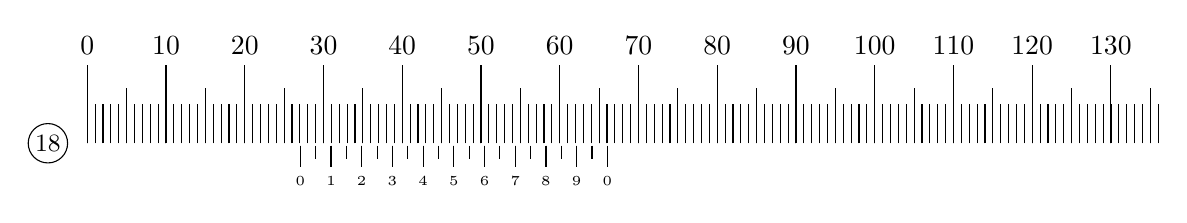
\begin{tikzpicture}

\node[circle, draw, minimum size=5mm, inner sep=0pt] (N) at (-0.5,0) {\small 18};

% Escala principal
	\foreach \x in {0.0, 0.1, ..., 13.7}
		\draw (\x,0) -- (\x,0.5);

	\foreach \x in {0, 0.5, ..., 13.5}
		\draw (\x,0) -- (\x,0.7);

	\draw (0,0) -- (0,1) node[anchor=south] {0};
	\foreach \x in {1, 2, ..., 13}
		\draw (\x,0) -- (\x,1) node[anchor=south] {\x0};

% Escala auxiliar
\begin{scope}[xshift=27.05mm]
	\foreach \x in {0.000, 0.195, ..., 3.89}
		\draw (\x,-0.03) -- (\x,-0.2);

	\foreach \x [count=\xi from 0] in {0, 0.39, ..., 3.89}
		\draw (\x,-0.03) -- (\x,-0.3) node[anchor=north] {\tiny \xi};
	
	\draw (3.9,-0.03) -- (3.9,-0.3) node[anchor=north] {\tiny 0};
\end{scope}
\end{tikzpicture}
\end{figure*}

\begin{figure*}
\centering
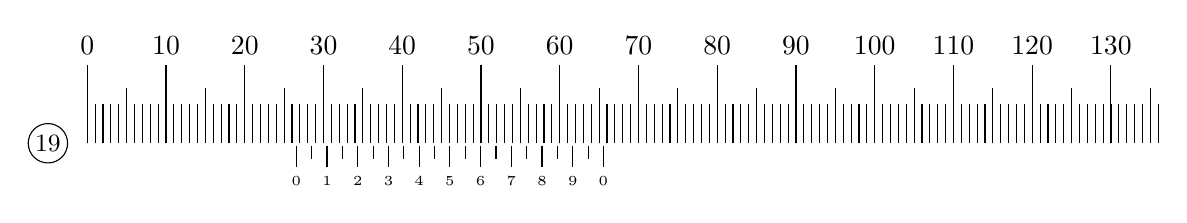
\begin{tikzpicture}

\node[circle, draw, minimum size=5mm, inner sep=0pt] (N) at (-0.5,0) {\small 19};

% Escala principal
	\foreach \x in {0.0, 0.1, ..., 13.7}
		\draw (\x,0) -- (\x,0.5);

	\foreach \x in {0, 0.5, ..., 13.5}
		\draw (\x,0) -- (\x,0.7);

	\draw (0,0) -- (0,1) node[anchor=south] {0};
	\foreach \x in {1, 2, ..., 13}
		\draw (\x,0) -- (\x,1) node[anchor=south] {\x0};

% Escala auxiliar
\begin{scope}[xshift=26.55mm]
	\foreach \x in {0.000, 0.195, ..., 3.89}
		\draw (\x,-0.03) -- (\x,-0.2);

	\foreach \x [count=\xi from 0] in {0, 0.39, ..., 3.89}
		\draw (\x,-0.03) -- (\x,-0.3) node[anchor=north] {\tiny \xi};
	
	\draw (3.9,-0.03) -- (3.9,-0.3) node[anchor=north] {\tiny 0};
\end{scope}
\end{tikzpicture}
\end{figure*}

\begin{figure*}
\centering
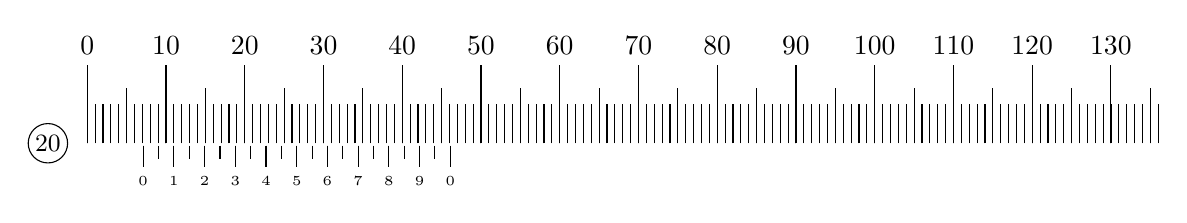
\begin{tikzpicture}

\node[circle, draw, minimum size=5mm, inner sep=0pt] (N) at (-0.5,0) {\small 20};

% Escala principal
	\foreach \x in {0.0, 0.1, ..., 13.7}
		\draw (\x,0) -- (\x,0.5);

	\foreach \x in {0, 0.5, ..., 13.5}
		\draw (\x,0) -- (\x,0.7);

	\draw (0,0) -- (0,1) node[anchor=south] {0};
	\foreach \x in {1, 2, ..., 13}
		\draw (\x,0) -- (\x,1) node[anchor=south] {\x0};

% Escala auxiliar
\begin{scope}[xshift=7.10mm]
	\foreach \x in {0.000, 0.195, ..., 3.89}
		\draw (\x,-0.03) -- (\x,-0.2);

	\foreach \x [count=\xi from 0] in {0, 0.39, ..., 3.89}
		\draw (\x,-0.03) -- (\x,-0.3) node[anchor=north] {\tiny \xi};
	
	\draw (3.9,-0.03) -- (3.9,-0.3) node[anchor=north] {\tiny 0};
\end{scope}
\end{tikzpicture}
\end{figure*}

%%%%%%%%%%%%%%%%%%%%%%%%%%%%%

\begin{figure*}
\centering
\begin{tikzpicture}[scale=1.7]

	\node[circle, draw, minimum size=5mm, inner sep=0pt] (N) at (-0.75,0) {\small 21};

	\pgfmathsetmacro{\reading}{5.731} % leitura em mm
	
	\pgfmathsetmacro{\decimalpart}{\reading - int(\reading)}  % Extract decimal part
	\pgfmathsetmacro{\scaleddecimal}{\decimalpart * 100}  % Multiply by 100
	\pgfmathsetmacro{\yshift}{mod(\scaleddecimal, 50)}
	\pgfmathsetmacro{\clipsize}{\reading + 10}

	\clip (-0.5,1) rectangle (\clipsize mm,-1);
	
% Escala principal

	\draw (-0.4,0) -- (7,0);
	
	\foreach \x in {0.0, 0.1, ..., 7.0}
		\draw (\x,-0.05) -- (\x,-0.15);

	\foreach \x in {0, 5, ..., 70}
		\draw (\x mm,-0.05) -- (\x mm,-0.3)node[below]{\tiny \x};

	\foreach \x in {0.05, 0.15, ..., 7.0}
		\draw (\x,0.05) -- (\x,0.15);

% Escala auxiliar
	\begin{scope}[xshift=\reading mm]
		\fill[white] (0,-1) rectangle (1,1);
		\draw[gray] (0,-1) -- (0,1);
		
		\begin{scope}[yshift=-\yshift mm]
			\foreach \y in {0, 1, ...,49}
				\draw (0,\y mm) -- (2 mm,\y mm);

			\foreach \y in {0, 5, ..., 49}{
				%\pgfmathsetmacro{\newy}{int(\y + 10)}
				\draw (0,\y mm) -- (4 mm,\y mm) node[right]{\tiny \y};
			}
			
			\foreach \y in {0, 1, ..., 50}{
				\pgfmathsetmacro{\newy}{int(\y + 50)}
				\draw (0,\newy mm) -- (2 mm,\newy mm);
			}

			\foreach \y in {0, 5, ..., 50}{
				\pgfmathsetmacro{\newy}{int(\y + 50)}
				\draw (0,\newy mm) -- (4 mm,\newy mm) node[right]{\tiny \y};
			}
			
			\foreach \y in {0, 1, ..., 49}{
				\pgfmathsetmacro{\newy}{int(\y - 50)}
				\draw (0,\newy mm) -- (2 mm,\newy mm);
			}
			\foreach \y in {0, 5, ..., 49}{
				\pgfmathsetmacro{\newy}{int(\y - 50)}
				\draw (0,\newy mm) -- (4 mm,\newy mm) node[right]{\tiny \y};
			}
		\end{scope}
	
		\fill[color=white,path fading=south] (0,0) rectangle (1,1.2);
		\fill[color=white,path fading=north] (0,0) rectangle (1,-1.2);
		
	\end{scope}
\end{tikzpicture}
\end{figure*}

\begin{figure*}
\centering
\begin{tikzpicture}[scale=1.7]

	\node[circle, draw, minimum size=5mm, inner sep=0pt] (N) at (-0.75,0) {\small 22};
	
	\pgfmathsetmacro{\reading}{68.204} % leitura em mm
	
	\pgfmathsetmacro{\decimalpart}{\reading - int(\reading)}  % Extract decimal part
	\pgfmathsetmacro{\scaleddecimal}{\decimalpart * 100}  % Multiply by 100
	\pgfmathsetmacro{\yshift}{mod(\scaleddecimal, 50)}
	\pgfmathsetmacro{\clipsize}{\reading + 10}

	\clip (-0.5,1) rectangle (\clipsize mm,-1);
	
% Escala principal

	\draw (-0.4,0) -- (7,0);
	
	\foreach \x in {0.0, 0.1, ..., 7.0}
		\draw (\x,-0.05) -- (\x,-0.15);

	\foreach \x in {0, 5, ..., 70}
		\draw (\x mm,-0.05) -- (\x mm,-0.3)node[below]{\tiny \x};

	\foreach \x in {0.05, 0.15, ..., 7.0}
		\draw (\x,0.05) -- (\x,0.15);

% Escala auxiliar
	\begin{scope}[xshift=\reading mm]
		\fill[white] (0,-1) rectangle (1,1);
		\draw[gray] (0,-1) -- (0,1);
		
		\begin{scope}[yshift=-\yshift mm]
			\foreach \y in {0, 1, ...,49}
				\draw (0,\y mm) -- (2 mm,\y mm);

			\foreach \y in {0, 5, ..., 49}{
				%\pgfmathsetmacro{\newy}{int(\y + 10)}
				\draw (0,\y mm) -- (4 mm,\y mm) node[right]{\tiny \y};
			}
			
			\foreach \y in {0, 1, ..., 50}{
				\pgfmathsetmacro{\newy}{int(\y + 50)}
				\draw (0,\newy mm) -- (2 mm,\newy mm);
			}

			\foreach \y in {0, 5, ..., 50}{
				\pgfmathsetmacro{\newy}{int(\y + 50)}
				\draw (0,\newy mm) -- (4 mm,\newy mm) node[right]{\tiny \y};
			}
			
			\foreach \y in {0, 1, ..., 49}{
				\pgfmathsetmacro{\newy}{int(\y - 50)}
				\draw (0,\newy mm) -- (2 mm,\newy mm);
			}
			\foreach \y in {0, 5, ..., 49}{
				\pgfmathsetmacro{\newy}{int(\y - 50)}
				\draw (0,\newy mm) -- (4 mm,\newy mm) node[right]{\tiny \y};
			}
		\end{scope}
	
		\fill[color=white,path fading=south] (0,0) rectangle (1,1.2);
		\fill[color=white,path fading=north] (0,0) rectangle (1,-1.2);
		
	\end{scope}
\end{tikzpicture}
\end{figure*}

\begin{figure*}
\centering
\begin{tikzpicture}[scale=1.7]

	\node[circle, draw, minimum size=5mm, inner sep=0pt] (N) at (-0.75,0) {\small 23};
	
	\pgfmathsetmacro{\reading}{42.987} % leitura em mm
	
	\pgfmathsetmacro{\decimalpart}{\reading - int(\reading)}  % Extract decimal part
	\pgfmathsetmacro{\scaleddecimal}{\decimalpart * 100}  % Multiply by 100
	\pgfmathsetmacro{\yshift}{mod(\scaleddecimal, 50)}
	\pgfmathsetmacro{\clipsize}{\reading + 10}

	\clip (-0.5,1) rectangle (\clipsize mm,-1);
	
% Escala principal

	\draw (-0.4,0) -- (7,0);
	
	\foreach \x in {0.0, 0.1, ..., 7.0}
		\draw (\x,-0.05) -- (\x,-0.15);

	\foreach \x in {0, 5, ..., 70}
		\draw (\x mm,-0.05) -- (\x mm,-0.3)node[below]{\tiny \x};

	\foreach \x in {0.05, 0.15, ..., 7.0}
		\draw (\x,0.05) -- (\x,0.15);

% Escala auxiliar
	\begin{scope}[xshift=\reading mm]
		\fill[white] (0,-1) rectangle (1,1);
		\draw[gray] (0,-1) -- (0,1);
		
		\begin{scope}[yshift=-\yshift mm]
			\foreach \y in {0, 1, ...,49}
				\draw (0,\y mm) -- (2 mm,\y mm);

			\foreach \y in {0, 5, ..., 49}{
				%\pgfmathsetmacro{\newy}{int(\y + 10)}
				\draw (0,\y mm) -- (4 mm,\y mm) node[right]{\tiny \y};
			}
			
			\foreach \y in {0, 1, ..., 50}{
				\pgfmathsetmacro{\newy}{int(\y + 50)}
				\draw (0,\newy mm) -- (2 mm,\newy mm);
			}

			\foreach \y in {0, 5, ..., 50}{
				\pgfmathsetmacro{\newy}{int(\y + 50)}
				\draw (0,\newy mm) -- (4 mm,\newy mm) node[right]{\tiny \y};
			}
			
			\foreach \y in {0, 1, ..., 49}{
				\pgfmathsetmacro{\newy}{int(\y - 50)}
				\draw (0,\newy mm) -- (2 mm,\newy mm);
			}
			\foreach \y in {0, 5, ..., 49}{
				\pgfmathsetmacro{\newy}{int(\y - 50)}
				\draw (0,\newy mm) -- (4 mm,\newy mm) node[right]{\tiny \y};
			}
		\end{scope}
	
		\fill[color=white,path fading=south] (0,0) rectangle (1,1.2);
		\fill[color=white,path fading=north] (0,0) rectangle (1,-1.2);
		
	\end{scope}
\end{tikzpicture}
\end{figure*}

\begin{figure*}
\centering
\begin{tikzpicture}[scale=1.7]

	\node[circle, draw, minimum size=5mm, inner sep=0pt] (N) at (-0.75,0) {\small 24};
	
	\pgfmathsetmacro{\reading}{11.356} % leitura em mm
	
	\pgfmathsetmacro{\decimalpart}{\reading - int(\reading)}  % Extract decimal part
	\pgfmathsetmacro{\scaleddecimal}{\decimalpart * 100}  % Multiply by 100
	\pgfmathsetmacro{\yshift}{mod(\scaleddecimal, 50)}
	\pgfmathsetmacro{\clipsize}{\reading + 10}

	\clip (-0.5,1) rectangle (\clipsize mm,-1);
	
% Escala principal

	\draw (-0.4,0) -- (7,0);
	
	\foreach \x in {0.0, 0.1, ..., 7.0}
		\draw (\x,-0.05) -- (\x,-0.15);

	\foreach \x in {0, 5, ..., 70}
		\draw (\x mm,-0.05) -- (\x mm,-0.3)node[below]{\tiny \x};

	\foreach \x in {0.05, 0.15, ..., 7.0}
		\draw (\x,0.05) -- (\x,0.15);

% Escala auxiliar
	\begin{scope}[xshift=\reading mm]
		\fill[white] (0,-1) rectangle (1,1);
		\draw[gray] (0,-1) -- (0,1);
		
		\begin{scope}[yshift=-\yshift mm]
			\foreach \y in {0, 1, ...,49}
				\draw (0,\y mm) -- (2 mm,\y mm);

			\foreach \y in {0, 5, ..., 49}{
				%\pgfmathsetmacro{\newy}{int(\y + 10)}
				\draw (0,\y mm) -- (4 mm,\y mm) node[right]{\tiny \y};
			}
			
			\foreach \y in {0, 1, ..., 50}{
				\pgfmathsetmacro{\newy}{int(\y + 50)}
				\draw (0,\newy mm) -- (2 mm,\newy mm);
			}

			\foreach \y in {0, 5, ..., 50}{
				\pgfmathsetmacro{\newy}{int(\y + 50)}
				\draw (0,\newy mm) -- (4 mm,\newy mm) node[right]{\tiny \y};
			}
			
			\foreach \y in {0, 1, ..., 49}{
				\pgfmathsetmacro{\newy}{int(\y - 50)}
				\draw (0,\newy mm) -- (2 mm,\newy mm);
			}
			\foreach \y in {0, 5, ..., 49}{
				\pgfmathsetmacro{\newy}{int(\y - 50)}
				\draw (0,\newy mm) -- (4 mm,\newy mm) node[right]{\tiny \y};
			}
		\end{scope}
	
		\fill[color=white,path fading=south] (0,0) rectangle (1,1.2);
		\fill[color=white,path fading=north] (0,0) rectangle (1,-1.2);
		
	\end{scope}
\end{tikzpicture}
\end{figure*}

\begin{figure*}
\centering
\begin{tikzpicture}[scale=1.7]

	\node[circle, draw, minimum size=5mm, inner sep=0pt] (N) at (-0.75,0) {\small 25};
	
	\pgfmathsetmacro{\reading}{27.843} % leitura em mm
	
	\pgfmathsetmacro{\decimalpart}{\reading - int(\reading)}  % Extract decimal part
	\pgfmathsetmacro{\scaleddecimal}{\decimalpart * 100}  % Multiply by 100
	\pgfmathsetmacro{\yshift}{mod(\scaleddecimal, 50)}
	\pgfmathsetmacro{\clipsize}{\reading + 10}

	\clip (-0.5,1) rectangle (\clipsize mm,-1);
	
% Escala principal

	\draw (-0.4,0) -- (7,0);
	
	\foreach \x in {0.0, 0.1, ..., 7.0}
		\draw (\x,-0.05) -- (\x,-0.15);

	\foreach \x in {0, 5, ..., 70}
		\draw (\x mm,-0.05) -- (\x mm,-0.3)node[below]{\tiny \x};

	\foreach \x in {0.05, 0.15, ..., 7.0}
		\draw (\x,0.05) -- (\x,0.15);

% Escala auxiliar
	\begin{scope}[xshift=\reading mm]
		\fill[white] (0,-1) rectangle (1,1);
		\draw[gray] (0,-1) -- (0,1);
		
		\begin{scope}[yshift=-\yshift mm]
			\foreach \y in {0, 1, ...,49}
				\draw (0,\y mm) -- (2 mm,\y mm);

			\foreach \y in {0, 5, ..., 49}{
				%\pgfmathsetmacro{\newy}{int(\y + 10)}
				\draw (0,\y mm) -- (4 mm,\y mm) node[right]{\tiny \y};
			}
			
			\foreach \y in {0, 1, ..., 50}{
				\pgfmathsetmacro{\newy}{int(\y + 50)}
				\draw (0,\newy mm) -- (2 mm,\newy mm);
			}

			\foreach \y in {0, 5, ..., 50}{
				\pgfmathsetmacro{\newy}{int(\y + 50)}
				\draw (0,\newy mm) -- (4 mm,\newy mm) node[right]{\tiny \y};
			}
			
			\foreach \y in {0, 1, ..., 49}{
				\pgfmathsetmacro{\newy}{int(\y - 50)}
				\draw (0,\newy mm) -- (2 mm,\newy mm);
			}
			\foreach \y in {0, 5, ..., 49}{
				\pgfmathsetmacro{\newy}{int(\y - 50)}
				\draw (0,\newy mm) -- (4 mm,\newy mm) node[right]{\tiny \y};
			}
		\end{scope}
	
		\fill[color=white,path fading=south] (0,0) rectangle (1,1.2);
		\fill[color=white,path fading=north] (0,0) rectangle (1,-1.2);
		
	\end{scope}
\end{tikzpicture}
\end{figure*}

\begin{figure*}
\centering
\begin{tikzpicture}[scale=1.7]

	\node[circle, draw, minimum size=5mm, inner sep=0pt] (N) at (-0.75,0) {\small 26};
	
	\pgfmathsetmacro{\reading}{59.120} % leitura em mm
	
	\pgfmathsetmacro{\decimalpart}{\reading - int(\reading)}  % Extract decimal part
	\pgfmathsetmacro{\scaleddecimal}{\decimalpart * 100}  % Multiply by 100
	\pgfmathsetmacro{\yshift}{mod(\scaleddecimal, 50)}
	\pgfmathsetmacro{\clipsize}{\reading + 10}

	\clip (-0.5,1) rectangle (\clipsize mm,-1);
	
% Escala principal

	\draw (-0.4,0) -- (7,0);
	
	\foreach \x in {0.0, 0.1, ..., 7.0}
		\draw (\x,-0.05) -- (\x,-0.15);

	\foreach \x in {0, 5, ..., 70}
		\draw (\x mm,-0.05) -- (\x mm,-0.3)node[below]{\tiny \x};

	\foreach \x in {0.05, 0.15, ..., 7.0}
		\draw (\x,0.05) -- (\x,0.15);

% Escala auxiliar
	\begin{scope}[xshift=\reading mm]
		\fill[white] (0,-1) rectangle (1,1);
		\draw[gray] (0,-1) -- (0,1);
		
		\begin{scope}[yshift=-\yshift mm]
			\foreach \y in {0, 1, ...,49}
				\draw (0,\y mm) -- (2 mm,\y mm);

			\foreach \y in {0, 5, ..., 49}{
				%\pgfmathsetmacro{\newy}{int(\y + 10)}
				\draw (0,\y mm) -- (4 mm,\y mm) node[right]{\tiny \y};
			}
			
			\foreach \y in {0, 1, ..., 50}{
				\pgfmathsetmacro{\newy}{int(\y + 50)}
				\draw (0,\newy mm) -- (2 mm,\newy mm);
			}

			\foreach \y in {0, 5, ..., 50}{
				\pgfmathsetmacro{\newy}{int(\y + 50)}
				\draw (0,\newy mm) -- (4 mm,\newy mm) node[right]{\tiny \y};
			}
			
			\foreach \y in {0, 1, ..., 49}{
				\pgfmathsetmacro{\newy}{int(\y - 50)}
				\draw (0,\newy mm) -- (2 mm,\newy mm);
			}
			\foreach \y in {0, 5, ..., 49}{
				\pgfmathsetmacro{\newy}{int(\y - 50)}
				\draw (0,\newy mm) -- (4 mm,\newy mm) node[right]{\tiny \y};
			}
		\end{scope}
	
		\fill[color=white,path fading=south] (0,0) rectangle (1,1.2);
		\fill[color=white,path fading=north] (0,0) rectangle (1,-1.2);
		
	\end{scope}
\end{tikzpicture}
\end{figure*}

\begin{figure*}
\centering
\begin{tikzpicture}[scale=1.7]

	\node[circle, draw, minimum size=5mm, inner sep=0pt] (N) at (-0.75,0) {\small 27};
	
	\pgfmathsetmacro{\reading}{36.478} % leitura em mm
	
	\pgfmathsetmacro{\decimalpart}{\reading - int(\reading)}  % Extract decimal part
	\pgfmathsetmacro{\scaleddecimal}{\decimalpart * 100}  % Multiply by 100
	\pgfmathsetmacro{\yshift}{mod(\scaleddecimal, 50)}
	\pgfmathsetmacro{\clipsize}{\reading + 10}

	\clip (-0.5,1) rectangle (\clipsize mm,-1);
	
% Escala principal

	\draw (-0.4,0) -- (7,0);
	
	\foreach \x in {0.0, 0.1, ..., 7.0}
		\draw (\x,-0.05) -- (\x,-0.15);

	\foreach \x in {0, 5, ..., 70}
		\draw (\x mm,-0.05) -- (\x mm,-0.3)node[below]{\tiny \x};

	\foreach \x in {0.05, 0.15, ..., 7.0}
		\draw (\x,0.05) -- (\x,0.15);

% Escala auxiliar
	\begin{scope}[xshift=\reading mm]
		\fill[white] (0,-1) rectangle (1,1);
		\draw[gray] (0,-1) -- (0,1);
		
		\begin{scope}[yshift=-\yshift mm]
			\foreach \y in {0, 1, ...,49}
				\draw (0,\y mm) -- (2 mm,\y mm);

			\foreach \y in {0, 5, ..., 49}{
				%\pgfmathsetmacro{\newy}{int(\y + 10)}
				\draw (0,\y mm) -- (4 mm,\y mm) node[right]{\tiny \y};
			}
			
			\foreach \y in {0, 1, ..., 50}{
				\pgfmathsetmacro{\newy}{int(\y + 50)}
				\draw (0,\newy mm) -- (2 mm,\newy mm);
			}

			\foreach \y in {0, 5, ..., 50}{
				\pgfmathsetmacro{\newy}{int(\y + 50)}
				\draw (0,\newy mm) -- (4 mm,\newy mm) node[right]{\tiny \y};
			}
			
			\foreach \y in {0, 1, ..., 49}{
				\pgfmathsetmacro{\newy}{int(\y - 50)}
				\draw (0,\newy mm) -- (2 mm,\newy mm);
			}
			\foreach \y in {0, 5, ..., 49}{
				\pgfmathsetmacro{\newy}{int(\y - 50)}
				\draw (0,\newy mm) -- (4 mm,\newy mm) node[right]{\tiny \y};
			}
		\end{scope}
	
		\fill[color=white,path fading=south] (0,0) rectangle (1,1.2);
		\fill[color=white,path fading=north] (0,0) rectangle (1,-1.2);
		
	\end{scope}
\end{tikzpicture}
\end{figure*}

\begin{figure*}
\centering
\begin{tikzpicture}[scale=1.7]

	\node[circle, draw, minimum size=5mm, inner sep=0pt] (N) at (-0.75,0) {\small 28};
	
	\pgfmathsetmacro{\reading}{2.019} % leitura em mm
	
	\pgfmathsetmacro{\decimalpart}{\reading - int(\reading)}  % Extract decimal part
	\pgfmathsetmacro{\scaleddecimal}{\decimalpart * 100}  % Multiply by 100
	\pgfmathsetmacro{\yshift}{mod(\scaleddecimal, 50)}
	\pgfmathsetmacro{\clipsize}{\reading + 10}

	\clip (-0.5,1) rectangle (\clipsize mm,-1);
	
% Escala principal

	\draw (-0.4,0) -- (7,0);
	
	\foreach \x in {0.0, 0.1, ..., 7.0}
		\draw (\x,-0.05) -- (\x,-0.15);

	\foreach \x in {0, 5, ..., 70}
		\draw (\x mm,-0.05) -- (\x mm,-0.3)node[below]{\tiny \x};

	\foreach \x in {0.05, 0.15, ..., 7.0}
		\draw (\x,0.05) -- (\x,0.15);

% Escala auxiliar
	\begin{scope}[xshift=\reading mm]
		\fill[white] (0,-1) rectangle (1,1);
		\draw[gray] (0,-1) -- (0,1);
		
		\begin{scope}[yshift=-\yshift mm]
			\foreach \y in {0, 1, ...,49}
				\draw (0,\y mm) -- (2 mm,\y mm);

			\foreach \y in {0, 5, ..., 49}{
				%\pgfmathsetmacro{\newy}{int(\y + 10)}
				\draw (0,\y mm) -- (4 mm,\y mm) node[right]{\tiny \y};
			}
			
			\foreach \y in {0, 1, ..., 50}{
				\pgfmathsetmacro{\newy}{int(\y + 50)}
				\draw (0,\newy mm) -- (2 mm,\newy mm);
			}

			\foreach \y in {0, 5, ..., 50}{
				\pgfmathsetmacro{\newy}{int(\y + 50)}
				\draw (0,\newy mm) -- (4 mm,\newy mm) node[right]{\tiny \y};
			}
			
			\foreach \y in {0, 1, ..., 49}{
				\pgfmathsetmacro{\newy}{int(\y - 50)}
				\draw (0,\newy mm) -- (2 mm,\newy mm);
			}
			\foreach \y in {0, 5, ..., 49}{
				\pgfmathsetmacro{\newy}{int(\y - 50)}
				\draw (0,\newy mm) -- (4 mm,\newy mm) node[right]{\tiny \y};
			}
		\end{scope}
	
		\fill[color=white,path fading=south] (0,0) rectangle (1,1.2);
		\fill[color=white,path fading=north] (0,0) rectangle (1,-1.2);
		
	\end{scope}
\end{tikzpicture}
\end{figure*}

\begin{figure*}
\centering
\begin{tikzpicture}[scale=1.7]

	\node[circle, draw, minimum size=5mm, inner sep=0pt] (N) at (-0.75,0) {\small 29};
	
	\pgfmathsetmacro{\reading}{64.705} % leitura em mm
	
	\pgfmathsetmacro{\decimalpart}{\reading - int(\reading)}  % Extract decimal part
	\pgfmathsetmacro{\scaleddecimal}{\decimalpart * 100}  % Multiply by 100
	\pgfmathsetmacro{\yshift}{mod(\scaleddecimal, 50)}
	\pgfmathsetmacro{\clipsize}{\reading + 10}

	\clip (-0.5,1) rectangle (\clipsize mm,-1);
	
% Escala principal

	\draw (-0.4,0) -- (7,0);
	
	\foreach \x in {0.0, 0.1, ..., 7.0}
		\draw (\x,-0.05) -- (\x,-0.15);

	\foreach \x in {0, 5, ..., 70}
		\draw (\x mm,-0.05) -- (\x mm,-0.3)node[below]{\tiny \x};

	\foreach \x in {0.05, 0.15, ..., 7.0}
		\draw (\x,0.05) -- (\x,0.15);

% Escala auxiliar
	\begin{scope}[xshift=\reading mm]
		\fill[white] (0,-1) rectangle (1,1);
		\draw[gray] (0,-1) -- (0,1);
		
		\begin{scope}[yshift=-\yshift mm]
			\foreach \y in {0, 1, ...,49}
				\draw (0,\y mm) -- (2 mm,\y mm);

			\foreach \y in {0, 5, ..., 49}{
				%\pgfmathsetmacro{\newy}{int(\y + 10)}
				\draw (0,\y mm) -- (4 mm,\y mm) node[right]{\tiny \y};
			}
			
			\foreach \y in {0, 1, ..., 50}{
				\pgfmathsetmacro{\newy}{int(\y + 50)}
				\draw (0,\newy mm) -- (2 mm,\newy mm);
			}

			\foreach \y in {0, 5, ..., 50}{
				\pgfmathsetmacro{\newy}{int(\y + 50)}
				\draw (0,\newy mm) -- (4 mm,\newy mm) node[right]{\tiny \y};
			}
			
			\foreach \y in {0, 1, ..., 49}{
				\pgfmathsetmacro{\newy}{int(\y - 50)}
				\draw (0,\newy mm) -- (2 mm,\newy mm);
			}
			\foreach \y in {0, 5, ..., 49}{
				\pgfmathsetmacro{\newy}{int(\y - 50)}
				\draw (0,\newy mm) -- (4 mm,\newy mm) node[right]{\tiny \y};
			}
		\end{scope}
	
		\fill[color=white,path fading=south] (0,0) rectangle (1,1.2);
		\fill[color=white,path fading=north] (0,0) rectangle (1,-1.2);
		
	\end{scope}
\end{tikzpicture}
\end{figure*}

\begin{figure*}
\centering
\begin{tikzpicture}[scale=1.7]

	\node[circle, draw, minimum size=5mm, inner sep=0pt] (N) at (-0.75,0) {\small 30};
	
	\pgfmathsetmacro{\reading}{19.666} % leitura em mm
	
	\pgfmathsetmacro{\decimalpart}{\reading - int(\reading)}  % Extract decimal part
	\pgfmathsetmacro{\scaleddecimal}{\decimalpart * 100}  % Multiply by 100
	\pgfmathsetmacro{\yshift}{mod(\scaleddecimal, 50)}
	\pgfmathsetmacro{\clipsize}{\reading + 10}

	\clip (-0.5,1) rectangle (\clipsize mm,-1);
	
% Escala principal

	\draw (-0.4,0) -- (7,0);
	
	\foreach \x in {0.0, 0.1, ..., 7.0}
		\draw (\x,-0.05) -- (\x,-0.15);

	\foreach \x in {0, 5, ..., 70}
		\draw (\x mm,-0.05) -- (\x mm,-0.3)node[below]{\tiny \x};

	\foreach \x in {0.05, 0.15, ..., 7.0}
		\draw (\x,0.05) -- (\x,0.15);

% Escala auxiliar
	\begin{scope}[xshift=\reading mm]
		\fill[white] (0,-1) rectangle (1,1);
		\draw[gray] (0,-1) -- (0,1);
		
		\begin{scope}[yshift=-\yshift mm]
			\foreach \y in {0, 1, ...,49}
				\draw (0,\y mm) -- (2 mm,\y mm);

			\foreach \y in {0, 5, ..., 49}{
				%\pgfmathsetmacro{\newy}{int(\y + 10)}
				\draw (0,\y mm) -- (4 mm,\y mm) node[right]{\tiny \y};
			}
			
			\foreach \y in {0, 1, ..., 50}{
				\pgfmathsetmacro{\newy}{int(\y + 50)}
				\draw (0,\newy mm) -- (2 mm,\newy mm);
			}

			\foreach \y in {0, 5, ..., 50}{
				\pgfmathsetmacro{\newy}{int(\y + 50)}
				\draw (0,\newy mm) -- (4 mm,\newy mm) node[right]{\tiny \y};
			}
			
			\foreach \y in {0, 1, ..., 49}{
				\pgfmathsetmacro{\newy}{int(\y - 50)}
				\draw (0,\newy mm) -- (2 mm,\newy mm);
			}
			\foreach \y in {0, 5, ..., 49}{
				\pgfmathsetmacro{\newy}{int(\y - 50)}
				\draw (0,\newy mm) -- (4 mm,\newy mm) node[right]{\tiny \y};
			}
		\end{scope}
	
		\fill[color=white,path fading=south] (0,0) rectangle (1,1.2);
		\fill[color=white,path fading=north] (0,0) rectangle (1,-1.2);
		
	\end{scope}
\end{tikzpicture}
\end{figure*}

%%%%%%%%%%%%%%%%%%%%%%%%%%%%%%%%%%%

\begin{figure*}
\centering
\begin{tikzpicture}[scale=1.7]

	\node[circle, draw, minimum size=5mm, inner sep=0pt] (N) at (-0.75,0) {\small 31};
	
	\pgfmathsetmacro{\reading}{13.492} % leitura em mm
	
	\pgfmathsetmacro{\decimalpart}{\reading - int(\reading)}  % Extract decimal part
	\pgfmathsetmacro{\scaleddecimal}{\decimalpart * 100}  % Multiply by 100
	\pgfmathsetmacro{\yshift}{mod(\scaleddecimal, 50)}
	\pgfmathsetmacro{\clipsize}{\reading + 10}

	\clip (-0.5,1) rectangle (\clipsize mm,-1);
	
% Escala principal

	\draw (-0.4,0) -- (7,0);
	
	\foreach \x in {0.0, 0.1, ..., 7.0}
		\draw (\x,-0.05) -- (\x,-0.20);

	\foreach \x in {0, 5, ..., 70}
		\draw (\x mm,-0.05) -- (\x mm,-0.3)node[below]{\tiny \x};

	\foreach \x in {0.05, 0.15, ..., 7.0}
		\draw (\x,-0.05) -- (\x,-0.10);
	
	\foreach \y in {1, 3, ..., 9}
		\draw ($(-0.05,\y*0.09)$) -- ($(7,\y*0.09)$);
		
	\foreach \y in {2, 4, ..., 8}
		\draw ($(-0.05,\y*0.09)$) node[left]{\tiny \y} -- ($(7,\y*0.09)$);
		
	\draw (-0.05,0.9) node[left]{\tiny 0} -- (7,0.9);
		
		
% Escala auxiliar
	\begin{scope}[xshift=\reading mm]
		\fill[white] (0,-1) rectangle (1,1);
		\draw[gray] (0,-1) -- (0,1);
		
		\begin{scope}[yshift=-\yshift mm]
			\foreach \y in {0, 1, ...,49}
				\draw (0,\y mm) -- (2 mm,\y mm);

			\foreach \y in {0, 5, ..., 49}{
				%\pgfmathsetmacro{\newy}{int(\y + 10)}
				\draw (0,\y mm) -- (4 mm,\y mm) node[right]{\tiny \y};
			}
			
			\foreach \y in {0, 1, ..., 50}{
				\pgfmathsetmacro{\newy}{int(\y + 50)}
				\draw (0,\newy mm) -- (2 mm,\newy mm);
			}

			\foreach \y in {0, 5, ..., 50}{
				\pgfmathsetmacro{\newy}{int(\y + 50)}
				\draw (0,\newy mm) -- (4 mm,\newy mm) node[right]{\tiny \y};
			}
			
			\foreach \y in {0, 1, ..., 49}{
				\pgfmathsetmacro{\newy}{int(\y - 50)}
				\draw (0,\newy mm) -- (2 mm,\newy mm);
			}
			\foreach \y in {0, 5, ..., 49}{
				\pgfmathsetmacro{\newy}{int(\y - 50)}
				\draw (0,\newy mm) -- (4 mm,\newy mm) node[right]{\tiny \y};
			}
		\end{scope}
	
	\end{scope}
\end{tikzpicture}
\end{figure*}

\begin{figure*}
\centering
\begin{tikzpicture}[scale=1.7]

	\node[circle, draw, minimum size=5mm, inner sep=0pt] (N) at (-0.75,0) {\small 32};
	
	\pgfmathsetmacro{\reading}{47.816} % leitura em mm
	
	\pgfmathsetmacro{\decimalpart}{\reading - int(\reading)}  % Extract decimal part
	\pgfmathsetmacro{\scaleddecimal}{\decimalpart * 100}  % Multiply by 100
	\pgfmathsetmacro{\yshift}{mod(\scaleddecimal, 50)}
	\pgfmathsetmacro{\clipsize}{\reading + 10}

	\clip (-0.5,1) rectangle (\clipsize mm,-1);
	
% Escala principal

	\draw (-0.4,0) -- (7,0);
	
	\foreach \x in {0.0, 0.1, ..., 7.0}
		\draw (\x,-0.05) -- (\x,-0.20);

	\foreach \x in {0, 5, ..., 70}
		\draw (\x mm,-0.05) -- (\x mm,-0.3)node[below]{\tiny \x};

	\foreach \x in {0.05, 0.15, ..., 7.0}
		\draw (\x,-0.05) -- (\x,-0.10);
	
	\foreach \y in {1, 3, ..., 9}
		\draw ($(-0.05,\y*0.09)$) -- ($(7,\y*0.09)$);
		
	\foreach \y in {2, 4, ..., 8}
		\draw ($(-0.05,\y*0.09)$) node[left]{\tiny \y} -- ($(7,\y*0.09)$);
		
	\draw (-0.05,0.9) node[left]{\tiny 0} -- (7,0.9);
		
		
% Escala auxiliar
	\begin{scope}[xshift=\reading mm]
		\fill[white] (0,-1) rectangle (1,1);
		\draw[gray] (0,-1) -- (0,1);
		
		\begin{scope}[yshift=-\yshift mm]
			\foreach \y in {0, 1, ...,49}
				\draw (0,\y mm) -- (2 mm,\y mm);

			\foreach \y in {0, 5, ..., 49}{
				%\pgfmathsetmacro{\newy}{int(\y + 10)}
				\draw (0,\y mm) -- (4 mm,\y mm) node[right]{\tiny \y};
			}
			
			\foreach \y in {0, 1, ..., 50}{
				\pgfmathsetmacro{\newy}{int(\y + 50)}
				\draw (0,\newy mm) -- (2 mm,\newy mm);
			}

			\foreach \y in {0, 5, ..., 50}{
				\pgfmathsetmacro{\newy}{int(\y + 50)}
				\draw (0,\newy mm) -- (4 mm,\newy mm) node[right]{\tiny \y};
			}
			
			\foreach \y in {0, 1, ..., 49}{
				\pgfmathsetmacro{\newy}{int(\y - 50)}
				\draw (0,\newy mm) -- (2 mm,\newy mm);
			}
			\foreach \y in {0, 5, ..., 49}{
				\pgfmathsetmacro{\newy}{int(\y - 50)}
				\draw (0,\newy mm) -- (4 mm,\newy mm) node[right]{\tiny \y};
			}
		\end{scope}
	
	\end{scope}
\end{tikzpicture}
\end{figure*}

\begin{figure*}
\centering
\begin{tikzpicture}[scale=1.7]

	\node[circle, draw, minimum size=5mm, inner sep=0pt] (N) at (-0.75,0) {\small 33};
	
	\pgfmathsetmacro{\reading}{6.203} % leitura em mm
	
	\pgfmathsetmacro{\decimalpart}{\reading - int(\reading)}  % Extract decimal part
	\pgfmathsetmacro{\scaleddecimal}{\decimalpart * 100}  % Multiply by 100
	\pgfmathsetmacro{\yshift}{mod(\scaleddecimal, 50)}
	\pgfmathsetmacro{\clipsize}{\reading + 10}

	\clip (-0.5,1) rectangle (\clipsize mm,-1);
	
% Escala principal

	\draw (-0.4,0) -- (7,0);
	
	\foreach \x in {0.0, 0.1, ..., 7.0}
		\draw (\x,-0.05) -- (\x,-0.20);

	\foreach \x in {0, 5, ..., 70}
		\draw (\x mm,-0.05) -- (\x mm,-0.3)node[below]{\tiny \x};

	\foreach \x in {0.05, 0.15, ..., 7.0}
		\draw (\x,-0.05) -- (\x,-0.10);
	
	\foreach \y in {1, 3, ..., 9}
		\draw ($(-0.05,\y*0.09)$) -- ($(7,\y*0.09)$);
		
	\foreach \y in {2, 4, ..., 8}
		\draw ($(-0.05,\y*0.09)$) node[left]{\tiny \y} -- ($(7,\y*0.09)$);
		
	\draw (-0.05,0.9) node[left]{\tiny 0} -- (7,0.9);
		
		
% Escala auxiliar
	\begin{scope}[xshift=\reading mm]
		\fill[white] (0,-1) rectangle (1,1);
		\draw[gray] (0,-1) -- (0,1);
		
		\begin{scope}[yshift=-\yshift mm]
			\foreach \y in {0, 1, ...,49}
				\draw (0,\y mm) -- (2 mm,\y mm);

			\foreach \y in {0, 5, ..., 49}{
				%\pgfmathsetmacro{\newy}{int(\y + 10)}
				\draw (0,\y mm) -- (4 mm,\y mm) node[right]{\tiny \y};
			}
			
			\foreach \y in {0, 1, ..., 50}{
				\pgfmathsetmacro{\newy}{int(\y + 50)}
				\draw (0,\newy mm) -- (2 mm,\newy mm);
			}

			\foreach \y in {0, 5, ..., 50}{
				\pgfmathsetmacro{\newy}{int(\y + 50)}
				\draw (0,\newy mm) -- (4 mm,\newy mm) node[right]{\tiny \y};
			}
			
			\foreach \y in {0, 1, ..., 49}{
				\pgfmathsetmacro{\newy}{int(\y - 50)}
				\draw (0,\newy mm) -- (2 mm,\newy mm);
			}
			\foreach \y in {0, 5, ..., 49}{
				\pgfmathsetmacro{\newy}{int(\y - 50)}
				\draw (0,\newy mm) -- (4 mm,\newy mm) node[right]{\tiny \y};
			}
		\end{scope}
	
	\end{scope}
\end{tikzpicture}
\end{figure*}

\begin{figure*}
\centering
\begin{tikzpicture}[scale=1.7]

	\node[circle, draw, minimum size=5mm, inner sep=0pt] (N) at (-0.75,0) {\small 34};
	
	\pgfmathsetmacro{\reading}{69.774} % leitura em mm
	
	\pgfmathsetmacro{\decimalpart}{\reading - int(\reading)}  % Extract decimal part
	\pgfmathsetmacro{\scaleddecimal}{\decimalpart * 100}  % Multiply by 100
	\pgfmathsetmacro{\yshift}{mod(\scaleddecimal, 50)}
	\pgfmathsetmacro{\clipsize}{\reading + 10}

	\clip (-0.5,1) rectangle (\clipsize mm,-1);
	
% Escala principal

	\draw (-0.4,0) -- (7,0);
	
	\foreach \x in {0.0, 0.1, ..., 7.0}
		\draw (\x,-0.05) -- (\x,-0.20);

	\foreach \x in {0, 5, ..., 70}
		\draw (\x mm,-0.05) -- (\x mm,-0.3)node[below]{\tiny \x};

	\foreach \x in {0.05, 0.15, ..., 7.0}
		\draw (\x,-0.05) -- (\x,-0.10);
	
	\foreach \y in {1, 3, ..., 9}
		\draw ($(-0.05,\y*0.09)$) -- ($(7,\y*0.09)$);
		
	\foreach \y in {2, 4, ..., 8}
		\draw ($(-0.05,\y*0.09)$) node[left]{\tiny \y} -- ($(7,\y*0.09)$);
		
	\draw (-0.05,0.9) node[left]{\tiny 0} -- (7,0.9);
		
		
% Escala auxiliar
	\begin{scope}[xshift=\reading mm]
		\fill[white] (0,-1) rectangle (1,1);
		\draw[gray] (0,-1) -- (0,1);
		
		\begin{scope}[yshift=-\yshift mm]
			\foreach \y in {0, 1, ...,49}
				\draw (0,\y mm) -- (2 mm,\y mm);

			\foreach \y in {0, 5, ..., 49}{
				%\pgfmathsetmacro{\newy}{int(\y + 10)}
				\draw (0,\y mm) -- (4 mm,\y mm) node[right]{\tiny \y};
			}
			
			\foreach \y in {0, 1, ..., 50}{
				\pgfmathsetmacro{\newy}{int(\y + 50)}
				\draw (0,\newy mm) -- (2 mm,\newy mm);
			}

			\foreach \y in {0, 5, ..., 50}{
				\pgfmathsetmacro{\newy}{int(\y + 50)}
				\draw (0,\newy mm) -- (4 mm,\newy mm) node[right]{\tiny \y};
			}
			
			\foreach \y in {0, 1, ..., 49}{
				\pgfmathsetmacro{\newy}{int(\y - 50)}
				\draw (0,\newy mm) -- (2 mm,\newy mm);
			}
			\foreach \y in {0, 5, ..., 49}{
				\pgfmathsetmacro{\newy}{int(\y - 50)}
				\draw (0,\newy mm) -- (4 mm,\newy mm) node[right]{\tiny \y};
			}
		\end{scope}
	
	\end{scope}
\end{tikzpicture}
\end{figure*}

\begin{figure*}
\centering
\begin{tikzpicture}[scale=1.7]

	\node[circle, draw, minimum size=5mm, inner sep=0pt] (N) at (-0.75,0) {\small 35};
	
	\pgfmathsetmacro{\reading}{31.158} % leitura em mm
	
	\pgfmathsetmacro{\decimalpart}{\reading - int(\reading)}  % Extract decimal part
	\pgfmathsetmacro{\scaleddecimal}{\decimalpart * 100}  % Multiply by 100
	\pgfmathsetmacro{\yshift}{mod(\scaleddecimal, 50)}
	\pgfmathsetmacro{\clipsize}{\reading + 10}

	\clip (-0.5,1) rectangle (\clipsize mm,-1);
	
% Escala principal

	\draw (-0.4,0) -- (7,0);
	
	\foreach \x in {0.0, 0.1, ..., 7.0}
		\draw (\x,-0.05) -- (\x,-0.20);

	\foreach \x in {0, 5, ..., 70}
		\draw (\x mm,-0.05) -- (\x mm,-0.3)node[below]{\tiny \x};

	\foreach \x in {0.05, 0.15, ..., 7.0}
		\draw (\x,-0.05) -- (\x,-0.10);
	
	\foreach \y in {1, 3, ..., 9}
		\draw ($(-0.05,\y*0.09)$) -- ($(7,\y*0.09)$);
		
	\foreach \y in {2, 4, ..., 8}
		\draw ($(-0.05,\y*0.09)$) node[left]{\tiny \y} -- ($(7,\y*0.09)$);
		
	\draw (-0.05,0.9) node[left]{\tiny 0} -- (7,0.9);
		
		
% Escala auxiliar
	\begin{scope}[xshift=\reading mm]
		\fill[white] (0,-1) rectangle (1,1);
		\draw[gray] (0,-1) -- (0,1);
		
		\begin{scope}[yshift=-\yshift mm]
			\foreach \y in {0, 1, ...,49}
				\draw (0,\y mm) -- (2 mm,\y mm);

			\foreach \y in {0, 5, ..., 49}{
				%\pgfmathsetmacro{\newy}{int(\y + 10)}
				\draw (0,\y mm) -- (4 mm,\y mm) node[right]{\tiny \y};
			}
			
			\foreach \y in {0, 1, ..., 50}{
				\pgfmathsetmacro{\newy}{int(\y + 50)}
				\draw (0,\newy mm) -- (2 mm,\newy mm);
			}

			\foreach \y in {0, 5, ..., 50}{
				\pgfmathsetmacro{\newy}{int(\y + 50)}
				\draw (0,\newy mm) -- (4 mm,\newy mm) node[right]{\tiny \y};
			}
			
			\foreach \y in {0, 1, ..., 49}{
				\pgfmathsetmacro{\newy}{int(\y - 50)}
				\draw (0,\newy mm) -- (2 mm,\newy mm);
			}
			\foreach \y in {0, 5, ..., 49}{
				\pgfmathsetmacro{\newy}{int(\y - 50)}
				\draw (0,\newy mm) -- (4 mm,\newy mm) node[right]{\tiny \y};
			}
		\end{scope}
	
	\end{scope}
\end{tikzpicture}
\end{figure*}

\begin{figure*}
\centering
\begin{tikzpicture}[scale=1.7]

	\node[circle, draw, minimum size=5mm, inner sep=0pt] (N) at (-0.75,0) {\small 36};
	
	\pgfmathsetmacro{\reading}{22.947} % leitura em mm
	
	\pgfmathsetmacro{\decimalpart}{\reading - int(\reading)}  % Extract decimal part
	\pgfmathsetmacro{\scaleddecimal}{\decimalpart * 100}  % Multiply by 100
	\pgfmathsetmacro{\yshift}{mod(\scaleddecimal, 50)}
	\pgfmathsetmacro{\clipsize}{\reading + 10}

	\clip (-0.5,1) rectangle (\clipsize mm,-1);
	
% Escala principal

	\draw (-0.4,0) -- (7,0);
	
	\foreach \x in {0.0, 0.1, ..., 7.0}
		\draw (\x,-0.05) -- (\x,-0.20);

	\foreach \x in {0, 5, ..., 70}
		\draw (\x mm,-0.05) -- (\x mm,-0.3)node[below]{\tiny \x};

	\foreach \x in {0.05, 0.15, ..., 7.0}
		\draw (\x,-0.05) -- (\x,-0.10);
	
	\foreach \y in {1, 3, ..., 9}
		\draw ($(-0.05,\y*0.09)$) -- ($(7,\y*0.09)$);
		
	\foreach \y in {2, 4, ..., 8}
		\draw ($(-0.05,\y*0.09)$) node[left]{\tiny \y} -- ($(7,\y*0.09)$);
		
	\draw (-0.05,0.9) node[left]{\tiny 0} -- (7,0.9);
		
		
% Escala auxiliar
	\begin{scope}[xshift=\reading mm]
		\fill[white] (0,-1) rectangle (1,1);
		\draw[gray] (0,-1) -- (0,1);
		
		\begin{scope}[yshift=-\yshift mm]
			\foreach \y in {0, 1, ...,49}
				\draw (0,\y mm) -- (2 mm,\y mm);

			\foreach \y in {0, 5, ..., 49}{
				%\pgfmathsetmacro{\newy}{int(\y + 10)}
				\draw (0,\y mm) -- (4 mm,\y mm) node[right]{\tiny \y};
			}
			
			\foreach \y in {0, 1, ..., 50}{
				\pgfmathsetmacro{\newy}{int(\y + 50)}
				\draw (0,\newy mm) -- (2 mm,\newy mm);
			}

			\foreach \y in {0, 5, ..., 50}{
				\pgfmathsetmacro{\newy}{int(\y + 50)}
				\draw (0,\newy mm) -- (4 mm,\newy mm) node[right]{\tiny \y};
			}
			
			\foreach \y in {0, 1, ..., 49}{
				\pgfmathsetmacro{\newy}{int(\y - 50)}
				\draw (0,\newy mm) -- (2 mm,\newy mm);
			}
			\foreach \y in {0, 5, ..., 49}{
				\pgfmathsetmacro{\newy}{int(\y - 50)}
				\draw (0,\newy mm) -- (4 mm,\newy mm) node[right]{\tiny \y};
			}
		\end{scope}
	
	\end{scope}
\end{tikzpicture}
\end{figure*}

\begin{figure*}
\centering
\begin{tikzpicture}[scale=1.7]

	\node[circle, draw, minimum size=5mm, inner sep=0pt] (N) at (-0.75,0) {\small 37};
	
	\pgfmathsetmacro{\reading}{55.320} % leitura em mm
	
	\pgfmathsetmacro{\decimalpart}{\reading - int(\reading)}  % Extract decimal part
	\pgfmathsetmacro{\scaleddecimal}{\decimalpart * 100}  % Multiply by 100
	\pgfmathsetmacro{\yshift}{mod(\scaleddecimal, 50)}
	\pgfmathsetmacro{\clipsize}{\reading + 10}

	\clip (-0.5,1) rectangle (\clipsize mm,-1);
	
% Escala principal

	\draw (-0.4,0) -- (7,0);
	
	\foreach \x in {0.0, 0.1, ..., 7.0}
		\draw (\x,-0.05) -- (\x,-0.20);

	\foreach \x in {0, 5, ..., 70}
		\draw (\x mm,-0.05) -- (\x mm,-0.3)node[below]{\tiny \x};

	\foreach \x in {0.05, 0.15, ..., 7.0}
		\draw (\x,-0.05) -- (\x,-0.10);
	
	\foreach \y in {1, 3, ..., 9}
		\draw ($(-0.05,\y*0.09)$) -- ($(7,\y*0.09)$);
		
	\foreach \y in {2, 4, ..., 8}
		\draw ($(-0.05,\y*0.09)$) node[left]{\tiny \y} -- ($(7,\y*0.09)$);
		
	\draw (-0.05,0.9) node[left]{\tiny 0} -- (7,0.9);
		
		
% Escala auxiliar
	\begin{scope}[xshift=\reading mm]
		\fill[white] (0,-1) rectangle (1,1);
		\draw[gray] (0,-1) -- (0,1);
		
		\begin{scope}[yshift=-\yshift mm]
			\foreach \y in {0, 1, ...,49}
				\draw (0,\y mm) -- (2 mm,\y mm);

			\foreach \y in {0, 5, ..., 49}{
				%\pgfmathsetmacro{\newy}{int(\y + 10)}
				\draw (0,\y mm) -- (4 mm,\y mm) node[right]{\tiny \y};
			}
			
			\foreach \y in {0, 1, ..., 50}{
				\pgfmathsetmacro{\newy}{int(\y + 50)}
				\draw (0,\newy mm) -- (2 mm,\newy mm);
			}

			\foreach \y in {0, 5, ..., 50}{
				\pgfmathsetmacro{\newy}{int(\y + 50)}
				\draw (0,\newy mm) -- (4 mm,\newy mm) node[right]{\tiny \y};
			}
			
			\foreach \y in {0, 1, ..., 49}{
				\pgfmathsetmacro{\newy}{int(\y - 50)}
				\draw (0,\newy mm) -- (2 mm,\newy mm);
			}
			\foreach \y in {0, 5, ..., 49}{
				\pgfmathsetmacro{\newy}{int(\y - 50)}
				\draw (0,\newy mm) -- (4 mm,\newy mm) node[right]{\tiny \y};
			}
		\end{scope}
	
	\end{scope}
\end{tikzpicture}
\end{figure*}

\begin{figure*}
\centering
\begin{tikzpicture}[scale=1.7]

	\node[circle, draw, minimum size=5mm, inner sep=0pt] (N) at (-0.75,0) {\small 38};
	
	\pgfmathsetmacro{\reading}{9.681} % leitura em mm
	
	\pgfmathsetmacro{\decimalpart}{\reading - int(\reading)}  % Extract decimal part
	\pgfmathsetmacro{\scaleddecimal}{\decimalpart * 100}  % Multiply by 100
	\pgfmathsetmacro{\yshift}{mod(\scaleddecimal, 50)}
	\pgfmathsetmacro{\clipsize}{\reading + 10}

	\clip (-0.5,1) rectangle (\clipsize mm,-1);
	
% Escala principal

	\draw (-0.4,0) -- (7,0);
	
	\foreach \x in {0.0, 0.1, ..., 7.0}
		\draw (\x,-0.05) -- (\x,-0.20);

	\foreach \x in {0, 5, ..., 70}
		\draw (\x mm,-0.05) -- (\x mm,-0.3)node[below]{\tiny \x};

	\foreach \x in {0.05, 0.15, ..., 7.0}
		\draw (\x,-0.05) -- (\x,-0.10);
	
	\foreach \y in {1, 3, ..., 9}
		\draw ($(-0.05,\y*0.09)$) -- ($(7,\y*0.09)$);
		
	\foreach \y in {2, 4, ..., 8}
		\draw ($(-0.05,\y*0.09)$) node[left]{\tiny \y} -- ($(7,\y*0.09)$);
		
	\draw (-0.05,0.9) node[left]{\tiny 0} -- (7,0.9);
		
		
% Escala auxiliar
	\begin{scope}[xshift=\reading mm]
		\fill[white] (0,-1) rectangle (1,1);
		\draw[gray] (0,-1) -- (0,1);
		
		\begin{scope}[yshift=-\yshift mm]
			\foreach \y in {0, 1, ...,49}
				\draw (0,\y mm) -- (2 mm,\y mm);

			\foreach \y in {0, 5, ..., 49}{
				%\pgfmathsetmacro{\newy}{int(\y + 10)}
				\draw (0,\y mm) -- (4 mm,\y mm) node[right]{\tiny \y};
			}
			
			\foreach \y in {0, 1, ..., 50}{
				\pgfmathsetmacro{\newy}{int(\y + 50)}
				\draw (0,\newy mm) -- (2 mm,\newy mm);
			}

			\foreach \y in {0, 5, ..., 50}{
				\pgfmathsetmacro{\newy}{int(\y + 50)}
				\draw (0,\newy mm) -- (4 mm,\newy mm) node[right]{\tiny \y};
			}
			
			\foreach \y in {0, 1, ..., 49}{
				\pgfmathsetmacro{\newy}{int(\y - 50)}
				\draw (0,\newy mm) -- (2 mm,\newy mm);
			}
			\foreach \y in {0, 5, ..., 49}{
				\pgfmathsetmacro{\newy}{int(\y - 50)}
				\draw (0,\newy mm) -- (4 mm,\newy mm) node[right]{\tiny \y};
			}
		\end{scope}
	
	\end{scope}
\end{tikzpicture}
\end{figure*}

\begin{figure*}
\centering
\begin{tikzpicture}[scale=1.7]

	\node[circle, draw, minimum size=5mm, inner sep=0pt] (N) at (-0.75,0) {\small 39};
	
	\pgfmathsetmacro{\reading}{38.506} % leitura em mm
	
	\pgfmathsetmacro{\decimalpart}{\reading - int(\reading)}  % Extract decimal part
	\pgfmathsetmacro{\scaleddecimal}{\decimalpart * 100}  % Multiply by 100
	\pgfmathsetmacro{\yshift}{mod(\scaleddecimal, 50)}
	\pgfmathsetmacro{\clipsize}{\reading + 10}

	\clip (-0.5,1) rectangle (\clipsize mm,-1);
	
% Escala principal

	\draw (-0.4,0) -- (7,0);
	
	\foreach \x in {0.0, 0.1, ..., 7.0}
		\draw (\x,-0.05) -- (\x,-0.20);

	\foreach \x in {0, 5, ..., 70}
		\draw (\x mm,-0.05) -- (\x mm,-0.3)node[below]{\tiny \x};

	\foreach \x in {0.05, 0.15, ..., 7.0}
		\draw (\x,-0.05) -- (\x,-0.10);
	
	\foreach \y in {1, 3, ..., 9}
		\draw ($(-0.05,\y*0.09)$) -- ($(7,\y*0.09)$);
		
	\foreach \y in {2, 4, ..., 8}
		\draw ($(-0.05,\y*0.09)$) node[left]{\tiny \y} -- ($(7,\y*0.09)$);
		
	\draw (-0.05,0.9) node[left]{\tiny 0} -- (7,0.9);
		
		
% Escala auxiliar
	\begin{scope}[xshift=\reading mm]
		\fill[white] (0,-1) rectangle (1,1);
		\draw[gray] (0,-1) -- (0,1);
		
		\begin{scope}[yshift=-\yshift mm]
			\foreach \y in {0, 1, ...,49}
				\draw (0,\y mm) -- (2 mm,\y mm);

			\foreach \y in {0, 5, ..., 49}{
				%\pgfmathsetmacro{\newy}{int(\y + 10)}
				\draw (0,\y mm) -- (4 mm,\y mm) node[right]{\tiny \y};
			}
			
			\foreach \y in {0, 1, ..., 50}{
				\pgfmathsetmacro{\newy}{int(\y + 50)}
				\draw (0,\newy mm) -- (2 mm,\newy mm);
			}

			\foreach \y in {0, 5, ..., 50}{
				\pgfmathsetmacro{\newy}{int(\y + 50)}
				\draw (0,\newy mm) -- (4 mm,\newy mm) node[right]{\tiny \y};
			}
			
			\foreach \y in {0, 1, ..., 49}{
				\pgfmathsetmacro{\newy}{int(\y - 50)}
				\draw (0,\newy mm) -- (2 mm,\newy mm);
			}
			\foreach \y in {0, 5, ..., 49}{
				\pgfmathsetmacro{\newy}{int(\y - 50)}
				\draw (0,\newy mm) -- (4 mm,\newy mm) node[right]{\tiny \y};
			}
		\end{scope}
	
	\end{scope}
\end{tikzpicture}
\end{figure*}

\begin{figure*}
\centering
\begin{tikzpicture}[scale=1.7]

	\node[circle, draw, minimum size=5mm, inner sep=0pt] (N) at (-0.75,0) {\small 40};
	
	\pgfmathsetmacro{\reading}{63.029} % leitura em mm
	
	\pgfmathsetmacro{\decimalpart}{\reading - int(\reading)}  % Extract decimal part
	\pgfmathsetmacro{\scaleddecimal}{\decimalpart * 100}  % Multiply by 100
	\pgfmathsetmacro{\yshift}{mod(\scaleddecimal, 50)}
	\pgfmathsetmacro{\clipsize}{\reading + 10}

	\clip (-0.5,1) rectangle (\clipsize mm,-1);
	
% Escala principal

	\draw (-0.4,0) -- (7,0);
	
	\foreach \x in {0.0, 0.1, ..., 7.0}
		\draw (\x,-0.05) -- (\x,-0.20);

	\foreach \x in {0, 5, ..., 70}
		\draw (\x mm,-0.05) -- (\x mm,-0.3)node[below]{\tiny \x};

	\foreach \x in {0.05, 0.15, ..., 7.0}
		\draw (\x,-0.05) -- (\x,-0.10);
	
	\foreach \y in {1, 3, ..., 9}
		\draw ($(-0.05,\y*0.09)$) -- ($(7,\y*0.09)$);
		
	\foreach \y in {2, 4, ..., 8}
		\draw ($(-0.05,\y*0.09)$) node[left]{\tiny \y} -- ($(7,\y*0.09)$);
		
	\draw (-0.05,0.9) node[left]{\tiny 0} -- (7,0.9);
		
		
% Escala auxiliar
	\begin{scope}[xshift=\reading mm]
		\fill[white] (0,-1) rectangle (1,1);
		\draw[gray] (0,-1) -- (0,1);
		
		\begin{scope}[yshift=-\yshift mm]
			\foreach \y in {0, 1, ...,49}
				\draw (0,\y mm) -- (2 mm,\y mm);

			\foreach \y in {0, 5, ..., 49}{
				%\pgfmathsetmacro{\newy}{int(\y + 10)}
				\draw (0,\y mm) -- (4 mm,\y mm) node[right]{\tiny \y};
			}
			
			\foreach \y in {0, 1, ..., 50}{
				\pgfmathsetmacro{\newy}{int(\y + 50)}
				\draw (0,\newy mm) -- (2 mm,\newy mm);
			}

			\foreach \y in {0, 5, ..., 50}{
				\pgfmathsetmacro{\newy}{int(\y + 50)}
				\draw (0,\newy mm) -- (4 mm,\newy mm) node[right]{\tiny \y};
			}
			
			\foreach \y in {0, 1, ..., 49}{
				\pgfmathsetmacro{\newy}{int(\y - 50)}
				\draw (0,\newy mm) -- (2 mm,\newy mm);
			}
			\foreach \y in {0, 5, ..., 49}{
				\pgfmathsetmacro{\newy}{int(\y - 50)}
				\draw (0,\newy mm) -- (4 mm,\newy mm) node[right]{\tiny \y};
			}
		\end{scope}
	
	\end{scope}
\end{tikzpicture}
\end{figure*}

\FloatBarrier
%%%%%%%%%%%%%%%%%%%%%%%%%%%%%%%%%%%%%%%%%%%%%
\subsection{Respostas dos exercícios ímpares}
%%%%%%%%%%%%%%%%%%%%%%%%%%%%%%%%%%%%%%%%%%%%%

\emph{Questão 1}
\begin{multicols}{2}
\begin{description}
	\item[1.] \np[cm]{15.7}
	\item[3.] \np[kg]{7.8}
	\item[5.] \np[m]{3,58}
	\item[7.] \np[L]{0.008}
	\item[9.] \np[m]{3.3}
	\item[11.] \np[m]{0.0042}
	\item[13.] \np[g]{3.13}
	\item[15.] \np[kg]{0.00057}
	\item[17.] \np[cm]{8,01}
	\item[19.] \np[g]{6,9E5}
\end{description}
\end{multicols}

\noindent\emph{Questão 2}
\begin{multicols}{2}
\begin{description}
	\item[1.] \np[m^2]{6.7}
	\item[3.] \np[kg]{27}
	\item[5.] \np[m]{3.5}
	\item[7.] \np[m/s^2]{0,70}
	\item[9.] \np[m/s^2]{2.55}
	\item[11.] \np[m]{0,75}
	\item[13.] \np[kg \cdot m/s^2]{1,0E2}
	\item[15.] \np[L]{3,30}
	\item[17.] \np[kg \cdot m^2]{107}
	\item[19.] \np[m]{6,0E2}
\end{description}
\end{multicols}

\noindent\emph{Questão 3}
\begin{multicols}{2}
\begin{description}
	\item[1.] \np{0,1819}
	\item[3.] \np{1,4E-2}
	\item[5.] \np{0,997}
	\item[7.] \np[m^{\nicefrac{1}{2}}]{1,9}
	\item[9.] \np{2.5E3}
\end{description}
\end{multicols}

\noindent\emph{Questão 4}
\begin{multicols}{2}
\begin{description}
	\item[1.] \np[m]{10}
	\item[3.] \np[kg]{11}
	\item[5.] \np[L]{5,4}
	\item[7.] \np[m/s^2]{29,4}
	\item[9.] \np[cm]{3,00}
\end{description}
\end{multicols}

\noindent\emph{Questão 5}
\begin{multicols}{2}
\begin{description}
	\item[1.] \np[m]{4,7}
	\item[3.] \np[kg \cdot m/s^2]{31,2}
	\item[5.] \np[L]{5,0}
	\item[7.] \np[m/s]{3,0}
	\item[9.] \np[cm]{9,42}
	\item[11.] \np[s]{1,9}
	\item[13.] \np[m]{4,50}
	\item[15.] \np[m]{3.6}
	\item[17.] \np[m^{-1}]{2,0}
	\item[19.] \np[m/s]{5,0}
\end{description}
\end{multicols}

\noindent\emph{Questão 6}
\begin{multicols}{2}
\begin{description}
	\item[1.] \np[mm]{47,24}
	\item[3.] \np[mm]{76.83}
	\item[5.] \np[mm]{58,16}
	\item[7.] \np[mm]{49,51}
	\item[9.] \np[mm]{65,72}
	\item[11.] \np[mm]{33.20}
	\item[13.] \np[mm]{12.45}
	\item[15.] \np[mm]{21.80}
	\item[17.] \np[mm]{9.35}
	\item[19.] \np[mm]{26.55}
	\item[21.] \np[mm]{5,731}
	\item[23.] \np[mm]{42,987}
	\item[25.] \np[mm]{27,843}
	\item[27.] \np[mm]{36,478}
	\item[29.] \np[mm]{64,705}
	\item[31.] \np[mm]{13,492}
	\item[33.] \np[mm]{6,203}
	\item[35.] \np[mm]{31,158}
	\item[37.] \np[mm]{55,320}
	\item[39.] \np[mm]{38,506}
\end{description}
\end{multicols}
